% define documentclass
\documentclass[12pt, bibliography=totoc, a4paper, abstracton, numbers=noenddot]{scrreprt}

% define used packages
\usepackage[left=4.0cm, right=2.0cm, top=3cm, bottom=3cm]{geometry}
\usepackage{bibgerm}
\usepackage[utf8]{inputenc}
\usepackage[T1]{fontenc}
\usepackage[pdftex]{graphicx}
\usepackage[ngerman]{babel}
\usepackage{lmodern}
\usepackage{listings}
\usepackage{includes/minted}
\usepackage[numbers]{natbib}

\bibliographystyle{alpha}

%\usepackage{tikz}
%\usetikzlibrary{shapes,arrows}
\usepackage{includes/pgf-umlsd}

\usepackage{lastpage}

%XXX: literatur links
%\usepackage{multibib} 
%\newcites{lit}{Bibliography} 


% advanced tables
\usepackage{array}

% header and footer
\usepackage{fancyhdr}

% links
\usepackage{url}

% internal links
\usepackage[colorlinks=true ,linkcolor=black,
			anchorcolor=black ,citecolor=black ,filecolor=black,
			menucolor=black ,urlcolor=black]{hyperref}

% mathematical formulas
\usepackage{amsmath, amssymb}

% to include images side by side
\usepackage{subfigure}

% define the programming language
\usepackage{listings}
\lstloadlanguages{Java,sh,bash,Haskell,HTML,PHP,XML}
\lstdefinelanguage{console}{
  morekeywords={},
  otherkeywords={warumgehtdasnicht>,\$}
}
\newcommand{\lstsetconsole}
{ \lstset{%language=sh,
        lineskip=-2pt,
        breaklines=true,
        language=console,
        breaklines=true,
        commentstyle=\textit,
        keywordstyle=\bfseries,
        basicstyle=\ttfamily,
        stringstyle=\ttfamily,
        showstringspaces=false,
        frame=single,
        tabsize=2
  }
}
\lstdefinelanguage{scalaconsole}{
  morekeywords={},
  otherkeywords={scala>,\|}
}
\newcommand{\lstsetrepl}
{ \lstset{%language=sh,
        lineskip=-2pt,
        breaklines=true,
        language=scalaconsole,
        breaklines=true,
        commentstyle=\textit,
        keywordstyle=\bfseries,
        basicstyle=\ttfamily,
        stringstyle=\ttfamily,
        showstringspaces=false,
        frame=single,
        tabsize=2
  }
}
\newcommand{\lstsetjava}{
 \lstset{language=Java,
        breaklines=true,
        commentstyle=\textit,
        keywordstyle=\bfseries,
        basicstyle=\ttfamily,
        stringstyle=\ttfamily,
        showstringspaces=false,
        frame=single,
        tabsize=2,
        literate=
        %linewidth=\textwidth,captionpos=b
        %numbers=left, stepnumber=5, numbersep=10pt
 }
}
\lstdefinelanguage{scala}{
  morekeywords={abstract,case,catch,class,def,%
    do,else,extends,false,final,finally,%
    for,forSome,if,implicit,import,lazy,match,mixin,%
    new,null,object,override,package,%
    private,protected,requires,return,sealed,%
    super,this,throw,trait,true,try,%
    type,val,var,while,with,yield},
  otherkeywords={_,:,=,=>,<-,<\%,<:,>:,\#,@},
  sensitive=true,
  morecomment=[l]{//},
  morecomment=[n]{/*}{*/},
  morestring=[b]",
  morestring=[b]',
  morestring=[b]"""
}
\newcommand{\lstsetscala}{
 \lstset{language=scala,
        breaklines=true,
        commentstyle=\textit,
        keywordstyle=\bfseries,
        basicstyle=\ttfamily,
        stringstyle=\ttfamily,
        showstringspaces=false,
        frame=single,
        tabsize=2
        %%linewidth=\textwidth,captionpos=b
        %numbers=left, stepnumber=5, numbersep=10pt
 }
}
\newcommand{\lstsethtml}{
 \lstset{language=HTML,
        breaklines=true,
        commentstyle=\textit,
        keywordstyle=\bfseries,
        basicstyle=\ttfamily,
        stringstyle=\ttfamily,
        showstringspaces=false,
        frame=single,
        tabsize=2
        %%linewidth=\textwidth,captionpos=b
        %numbers=left, stepnumber=5, numbersep=10pt
 }
}
\newcommand{\lstsetphp}{
 \lstset{language=PHP,
        breaklines=true,
        commentstyle=\textit,
        keywordstyle=\bfseries,
        basicstyle=\ttfamily,
        stringstyle=\ttfamily,
        showstringspaces=false,
        frame=single,
        tabsize=2
        %%linewidth=\textwidth,captionpos=b
        %numbers=left, stepnumber=5, numbersep=10pt
 }
}
\lstnewenvironment{code}
    {\lstset{}%
      \csname lst@SetFirstLabel\endcsname}
    {\csname lst@SaveFirstLabel\endcsname}
\newcommand{\lstsethaskell}{
    \lstset{
      language=Haskell,
      commentstyle=\textit,
      keywordstyle=\bfseries,
      basicstyle=\ttfamily,
      stringstyle=\ttfamily,
      showstringspaces=false,
      frame=single,
      flexiblecolumns=false,
      basewidth={0.5em,0.45em},
      literate={+}{{$+$}}1 {/}{{$/$}}1 {*}{{$*$}}1 {=}{{$=$}}1
               {==}{{$==$}}2 %{!=}{{$\not\equiv$}}2
               {>}{{$>$}}1 {<}{{$<$}}1 {\\}{{$\lambda$}}1
               {\\\\}{{\char`\\\char`\\}}1
               {->}{{$\rightarrow$} }2 {>=}{{$\geq$}}2 {<-}{{$\leftarrow$}}2
               {<=}{{$\leq$}}2 {=>}{{$\Rightarrow$} }2
               {\ .}{{$\circ$}}2 {\ .\ }{{$\circ$}}2 {(.)}{({$\circ$})}2
               {>>}{{>>}}2 {>>=}{{>>=}}2
               {|}{{$\mid$}}1
    }
}
\lstdefinelanguage{JavaScript}{
  keywords={typeof, new, true, false, catch,%
    function, return, null, catch, switch, var,%
    if, in, while, do, else, case, break},
  ndkeywords={class, export, boolean, throw, implements, import, this},
  sensitive=false,
  comment=[l]{//},
  morecomment=[s]{/*}{*/},
  morestring=[b]',
  morestring=[b]"
}
\newcommand{\lstsetjavascript}{
  \lstset{
		language=JavaScript,
		breaklines=true,
		commentstyle=\textit,
		basicstyle=\ttfamily,
		keywordstyle=\bfseries,
		stringstyle=\ttfamily,
		showstringspaces=false,
		frame=single,
		tabsize=2
  }
}
\newcommand{\lstsetxml}{
 \lstset{language=XML,
        breaklines=true,
        commentstyle=\sffamily,
        keywordstyle=\bfseries,
        basicstyle=\sffamily,
        showstringspaces=false,
        stringstyle=\ttfamily,
        frame=single,
        tabsize=2,
        literate=
        %linewidth=\textwidth,captionpos=b
        %numbers=left, stepnumber=5, numbersep=10pt
 }
}
\lstdefinelanguage{CSharp}{
 morekeywords = {abstract,event,new,struct,as,explicit,%
    null,switch,base,extern,object,this,bool,false,%
    operator,throw,break,finally,out,true,byte,fixed,%
    override,try,case,float,params,typeof,catch,for,%
    private,uint,char,foreach,protected,ulong,checked,%
    goto,public,unchecked,class,if,readonly,unsafe,%
    const,implicit,ref,ushort,continue,in,return,using,%
    decimal,int,sbyte,virtual,default,interface,sealed,%
    volatile,delegate,internal,short,void,do,is,sizeof,%
    while,double,lock,stackalloc,else,long,static,%
    enum,namespace,string,partial},
  morecomment = [l]{//},
  morecomment = [l]{///},
  morecomment = [s]{/*}{*/},
  morestring=[b]",
  sensitive = true
}
\newcommand{\lstsetcsharp}{
 \lstset{language=csharp,
        breaklines=true,
        commentstyle=\sffamily,
        basicstyle=\sffamily,
        keywordstyle=\bfseries,
        stringstyle=\ttfamily,
        showstringspaces=false,
        frame=single,
        tabsize=2
        %%linewidth=\textwidth,captionpos=b
        %numbers=left, stepnumber=5, numbersep=10pt
 }
}
\lstdefinelanguage{FSharp}{
  morekeywords={abstract,and,as,assert,base,begin,%
    class,default,delegate,do,done,downcast,downto,%
    elif,else,end,exception,extern,false,finally,for,fun,%
    function,if,in,inherit,inline,interface,internal,lazy,%
    let,match,member,module,mutable,namespace,%
    new,not,null,of,open,or,override,private,public,rec,%
    return,static,struct,then,to,true,try,type,upcast,use,%
    val,void,when,while,with,yield,asr,land,lor,lsl,lsr,lxor,%
    mod,sig,atomic,break,checked,component,const,%
    constraint,constructor,continue,eager,event,external,%
    fixed,functor,global,include,method,mixin,object,%
    parallel,process,protected,pure,sealed,tailcall,trait,virtual,volatile},     
  sensitive=false,
  morecomment=[l][\color{greencomments}]{///},
  morecomment=[l][\color{greencomments}]{//},
  morecomment=[s][\color{greencomments}]{{(*}{*)}},
  morestring=[b]"
}
\newcommand{\lstsetfsharp}{
 \lstset{language=fsharp,
        breaklines=true,
        commentstyle=\sffamily,
        basicstyle=\sffamily,
        keywordstyle=\bfseries,
        stringstyle=\ttfamily,
        showstringspaces=false,
        frame=single,
        tabsize=2
        %%linewidth=\textwidth,captionpos=b
        %numbers=left, stepnumber=5, numbersep=10pt
 }
}

%set default pagestyle
\pagestyle{empty}

\setlength{\parindent}{0pt}
\setlength{\parskip}{3pt}


% settings for development - 1 page per section
\usepackage{includes/pagedsections}
%\usepackage[doublespacing]{setspace}


% #####
% #
% # START config area
% #
% #####

\newcommand{\HEADER}[0]{Fachhochschule Schmalkalden WS 2012/2013}
\newcommand{\PAGENUMBERS}[0]{Seite \pagemark \ von \pageref{LastPage}}
\newcommand{\DATE}[0]{31.11.2012}

\newcommand{\AUTHOR}[0]{Ronny Pfannschmidt}
\newcommand{\MATNR}[0]{250154}
\newcommand{\STREET}[0]{Brunnenstr. 16}
\newcommand{\ZIP}[0]{98587}
\newcommand{\TOWN}[0]{Steinbach Hallenberg}

\newcommand{\REFERENT}[0]{Prof. Dr. Harm Kolle}
\newcommand{\KOREFERENT}[0]{Prof. Dr. David Sommer?!?!}

\newcommand{\TITLE}[0]{Kontinuierliche Integration}
\newcommand{\SUBTITLEA}[0]{Design und prototypische Implementation}
\newcommand{\SUBTITLEB}[0]{auf Basis einer Verteilten Datenbank}
\newcommand{\COURSE}[0]{Informatik}
\newcommand{\TYPE}[0]{Diplomarbeit}
\newcommand{\COMPLETION}[0]{Dipl. Ing. Informatik (FH)}

% #####
% #
% # END config area
% #
% #####

% starting the document
\begin{document}

% set pagenumbering to roman(I II III IV)
\pagenumbering{Roman}
% input the title
% #####
% # This is the titlelayout from Prof. Dr. Oliver Braun (Fachhochschule
% # Schmalkalden)
% #
% # if you want to use it, please comment the lower title layout 
% #  
% #####

% \author{
% \\[1em]
% an der Fachhochschule Schmalkalden\\
% Fakultät Informatik\\[2em]
%   Referent: \REFERENT\\
%   Koreferent: \COREFERENT\\[2em]
% eingereicht von:\\[1em]
% \AUTHOR\\
% Matrikel-Nr.: \MATNR\\
% \STREET\\
% \TOWN\\
% }
% \date{Schmalkalden, den \DATE}
% \title{\TITLE}
% \subtitle{
% \TYPE\\
% Zur Erlangung des akademischen Grades eines\\
% \COMPLETION
% }
%\maketitle

% #####
% #
% # Default layout
% #
% #####
\begin{titlepage}
  \begin{center}
  	\includegraphics[scale=0.15]{images/logo.jpg}
  \end{center}
  \vspace{40pt}
  \sffamily
  \begin{tabular}{|l>{\raggedright\hspace{0pt}\arraybackslash}p{15cm}}
    & \\
    & \large\textbf{\TYPE}\\[\baselineskip]
    & \huge\textbf{\TITLE}\\[\baselineskip]
    & \textbf{Zur Erlangung des akademischen Grades eines}\\ 
    & \COMPLETION\\
    & - \COURSE -\\
    & \\
  \end{tabular}
  \vfill
  \begin{tabular}{ll@{}}
    & Fakultät Informatik\\[\baselineskip]
    &   Referent: \REFERENT\\[\baselineskip]
    &   Korreferent: \KOREFERENT\\[\baselineskip]
    & \\[\baselineskip]
    & eingereicht von:\\[\baselineskip]
    & \AUTHOR\\[\baselineskip]
    & Matr.-Nr. \MATNR\\[\baselineskip]
    & \STREET\\[\baselineskip]
    & \ZIP \ \TOWN\\[\baselineskip]
    & \\[\baselineskip]
    & Schmalkalden, den \DATE\\[\baselineskip]
  \end{tabular}
\end{titlepage}


%XXX
%\begin{abstract}

Kontinuierliche Integration, Kontinuierliches Testen und Kontinuierliche Verteilung entwickeln sich in der modernen Softwareentwicklung immer mehr zu einem Unabdingbaren Werkzeug,
welches  maßgeblich bei der Früherkennung von Fehlern hilft.

Die Werkzeuge die diese Verfahren ermöglichen lassen jedoch einige Fragen und Probleme offen.
In dieser Arbeit werden diese Probleme zuerst erörtert. Anschließend werden Lösungswege auf Basis einer verteilten Datenbank vorgestellt
und als Prototyp implementiert.

Der Prototyp Wird dann evaluiert und optimiert.


\end{abstract}


% load the preamble
\renewcommand\abstractname{Danksagung}
\begin{abstract}
blabla\ldots
\end{abstract}


% loads the fancy pagestyle for register part
% set the pagestyle to fancy
\pagestyle{fancy}

\fancyhf{}% clear all fields
  % define the header
  \fancyhead[L]{\leftmark}% left header
  \fancyhead[R]{\HEADER}% right header
  \renewcommand{\headrulewidth}{0.4pt}% top line

  % define the footer
  \fancyfoot[L]{\AUTHOR}% left footer
  \fancyfoot[R]{\pagemark}% right footer
  \renewcommand{\footrulewidth}{0.6pt}% bottom line

  % redefine the chaptermark to have '1. Chaptername' and not 'CHAPTER 1.
  % CHAPTERNAME'
  \renewcommand{\chaptermark}[1]{\markboth{\thechapter.\ #1}{}}

% override the plain style
\fancypagestyle{plain}{%
\fancyhf{}% clear all fields
  % define the header
  \renewcommand{\headrulewidth}{0.0pt}% top line

  % define the footer
  \fancyfoot[L]{\AUTHOR}% left footer
  \fancyfoot[R]{\pagemark}% right footer
  \renewcommand{\footrulewidth}{0.6pt}% bottom line
}


% create the registers
\tableofcontents\newpage

% set pagenumbering to arabic(1 2 3 4)
\pagenumbering{arabic}
% loads the fancy pagestyle for main part
% set the pagestyle to fancy
\pagestyle{fancy}

\fancyhf{}% clear all fields
  % define the header
  \fancyhead[L]{\leftmark}% left header
  \fancyhead[R]{\HEADER}% right header
  \renewcommand{\headrulewidth}{0.4pt}% top line

  % define the footer
  \fancyfoot[L]{\AUTHOR}% left footer
  \fancyfoot[R]{\PAGENUMBERS}% right footer
  \renewcommand{\footrulewidth}{0.6pt}% bottom line

  % redefine the chaptermark to have '1. Chaptername' and not 'CHAPTER 1.
  % CHAPTERNAME'
  \renewcommand{\chaptermark}[1]{\markboth{\thechapter.\ #1}{}}

% override the plain style
\fancypagestyle{plain}{%
\fancyhf{}% clear all fields
  % define the header
  \renewcommand{\headrulewidth}{0pt}% top line

  % define the footer
  \fancyfoot[L]{\AUTHOR}% left footer
  \fancyfoot[R]{\PAGENUMBERS}% right footer
  \renewcommand{\footrulewidth}{0.6pt}% bottom line
}


% #####
% # load the chapter from the files
% #
% # TODO: create new chapter
% #####


\chapter{Einleitung (5\%) }
\label{chap:intro}
\section{Motivation}

Kontinuierliche Integration ist ein wachsender Bereich
in der Welt der Software-Entwicklung und ihrer Qualitätssicherung.

% referenzen folwer/xp
Entstammend aus der Praxis des ``Extreme Programming''
\cite{xp:explained, folwer:xp},
beschäftigen sich Werkzeuge für kontinuierliche Integration damit,
Programme nach einer vollzogenen Integration zu testen.

In regelmäßigen Abständen, wie z.B. nach einer erfolgreichen Integration oder nach Arbeitsschluss,
wird das Programm vorbereitet und getestet.
Dies unterstützt das rasche Auffinden von Fehlern
und informiert über den Zustand der Software.
Nach Abschluss eines solchen Testes stehen dann das Resultat
und ein Zustandsbericht zur Verfügung.

Im Laufe der Zeit hat sich der Inhalt der Zustandsberichte weiterentwickelt.
Waren es anfänglich nur spärliche Informationen über Erfolg bzw. Misserfolg,
so findet man heutzutage Mitschnitte verschiedener Datenquellen, Testergebnisse
\cite{jenkins:junitxml}, sowie detaillierte Informationen über die Umgebung des Tests.

Weiterhin entstand mit Zunehmenden Anforderungen an Portabilität über
verschiedenste Arten von Plattformen (z.B. Datenbanken oder Betriebssystemen)
die Notwendigkeit das System in mehr als nur einer Umgebung zu testen.

Auch die Verwaltung von Software hat sich geändert.
Während ursprünglich nur auf einem Zweig der Entwicklung gearbeitet und integriert wurde,
findet dies Dank moderner Quellcode-verwaltung jetzt in vielen Zweigen statt.
\cite{dvcs:vorteile, dvcs:entwicklungsmodelle}

Aufgrund dieser Entwicklung stehen immer mehr Daten und Informationen zur Verfügung,
und es erscheint überaus sinnvoll, diese auch zu nutzen, um den Entwicklungsprozess zu unterstützen.

%XXX woanders?
Besonders Interessant sind dabei feststellbare Unterschiede zwischen den Umgebungen,
sowie feststellbare Unterschiede zwischen verschiedenen Zweigen der Entwicklung.

%XXX: test vor integration?


%\begin{verbatim}
%start traditionelles ci
%ueberfuehrung anforderungen
%ueberfuehrung branches, build achsen
%groessere datenmengen
%analyse
%feststellung struktir
%\end{verbatim}



\section{Problem}

Die Zukunftsvision, die Daten zu nutzen,
trifft in der Praxis auf einige harte Probleme.
Existierende Systeme sind schwer erweiterbar und haben oft schwer zugängliche Datenmodelle.

Es gibt keine Standards für Schnittstellen um CI-Systeme zu erweitern und mit ihren Daten zu arbeiten

Die Kombination dieser beiden Problemen erzeugt wiederum viele Probleme,
welche später im Kapitel \ref{chap:ist-analyse} behandelt werden.

Das Resultat ist, dass die existierenden Systeme im Bezug auf die Zukunftsvisionen,
nicht oder nur schwer anzupassen sind.

Der Mangel an Schnittstellen für den Datenzugriff und
das Fehlen von Schnittstellen für die Erweiterung der CI-Systeme
erschwert die Implementation von Werkzeugen für Analyse ungemein.


\section{Zielsetzung}
%XXX nochmal
Ziel dieser Arbeit ist es  aufzuzeigen, dass die oben genannten Probleme lösbar sind.
Zu diesem Zweck soll der Kern für ein System geschaffen werden,
welches in der Lage ist dies umzusetzen.

Es ist somit ein verteiltes System für Kontinuierliche Integration zu schaffen,
welches auf Datenbanktechnik basiert.
Dies dient als Ansatzpunkt, um das System zu erweitern und
Schnittstellen für den Datenzugriff zur Verfügung zu stellen.

Dabei sollten sowohl die grundlegenden Funktionen eines CI,
als auch die Möglichkeit der Erweiterung in Betracht gezogen werden.
Beispiele für solche Erweiterungen wären, wie schon genannt,
vergleichende Analyse zwischen Entwicklung-zweigen oder eigenständige Analysewerkzeuge.

Wichtig ist hierbei die grundlegende Erweiterbarkeit aufzuzeigen
und nicht die Lösung eines speziellen Problems.

\section{Abgrenzung}

Es soll lediglich der \emph{Kern} eines Systems als \emph{Prototyp} geschaffen werden,
damit werden Punkte wie die Benutzeroberfläche und Benutzer-verwaltung
außen vor gestellt.

Um die Arbeit überschaubar zu halten, wird dabei darauf verzichtet, Analysewerkzeuge außerhalb der verwendeten Datenbank zu betrachten.
Stattdessen wird der Kern des Systems und die Datenbank in den Fokus gestellt.


\section{Aufbau der Arbeit}



\chapter{Grundlagen (5\%)}

Dieses Kapitel beschreibt einige Grundlagen

\section{CAP}
\label{sec:base:cap}


%XXX literatur

Das CAP Theorem beschreibt 3 Grundlegende

\begin{verbatim}
- basics - copy somewhere
\end{verbatim}

\section{BASE}

\section{Verteilte Systeme}

\begin{verbatim}
- basics - copy somewhere
\end{verbatim}

\section{Kontinuierliche Integration/Verteilung}
\label{sec:base:ci}
\begin{verbatim}

- folwer ci - grundlegende verwendung
- http://jayflowers.com/joomla/index.php?option=com_content&task=view&id=26
\end{verbatim}

\section{Sourcecode/Versions Management}

\begin{verbatim}
- git/hg?
- branches
- entwicklungsmodelle
\end{verbatim}

\chapter{Ist-Analyse ( 5 \%)}
\label{chap:ist-analyse}

Dieses Kapitel dient der Beschreibung existierender System.
Es soll ihre Eigenschaften und Probleme aufzeigen.
Diese werden zuerst Theoretisch betrachtet und
dann an Systemen in der Praxis demonstriert.

% dieses kap dient .. und damit soll .. aufbau

\section{Eigenschaften der existierenden Systeme}

\subsection{Struktur}
\label{sec:ist-analyse:struktur}

Wie in der folgenden Grafik leicht zu erkennen,
sind traditionellen CI-Systeme Client-Server Systeme.

\begin{figure}[ht]
  \centering
  \label{fig:ist-aufbau-tradition}
  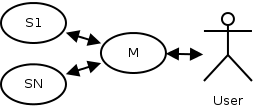
\includegraphics[height=1in]{imageinput/ist-aufbau-tradition.png}
  \caption{Logischer Aufbau eines CI System}
\end{figure}

Der sogenannte Master ist der Server und verwaltet alle Daten.
Die Slaves sind die Clients und verrichten die eigentliche Arbeit.
Sie sammeln Daten und liefern diese einschliesslich der Resultate beim Master ab.

Benutzer interagieren Ausschliesslich mit dem Master.

\subsection{Datensammlung}
Wie bereits in Sektion~\ref{sec:base:ci} erw\"ahnt,
f\"uhrt ein CI-System nicht nur Auftr\"age aus,
sondern sammelt auch daten f\"ur die sp\"atere Weiterverarbeitung.

Die Datensammlung l\"asst sich dabei grob in 2 Bereiche einteilen.
Zum einen die Laufzeitdaten und zum anderen die Artefakte.

Laufeitdaten fallen bereits w\"ahrend der Ausf\"uhrung an,
und beinhalten in der Regel zumindest die Textuellen Ausgaben
der ausgef\"uhrten Programme.
Weitere M\"oglichkeiten k\"onnen Testresultate, echzeit Logs und Ausf\"uhrungsstatistiken sein.
Laufzeitdaten werden dem Benutzer in idr. Zeitnah zur Verf\"ugung gestellt.

Artefakte hingegen sind Dateien,
welche erst nach Abschluss eines Schrittes zur verf\"ugung stehen.
Zu ihnen geh\"oren neben den traditionellen ausf\"uhrbaren Dateien
auch lauff\"ahige Archive des Gesammtprogrammes oder Testergebnisse in Formaten wie z.b. JunitXML oder TAP.

%XXX: cite tap, junitxml

Diese werden zum Master geschickt, dort aufbewahrt und sp\"ater genutzt.

In der Regel werden ausf\"uhrbare Artefakte zum Download angeboten,
w\"ahrend Testergebnisse nur dargestellt werden.


\section{Probleme existierender Systeme}

Diese Sektion gibt einen \"Uberblick \"uber die Problemarten existierender Ststeme

\subsection{Datenzugriff}

Beim Datenzugriff sind die existierenden Systeme besonders Problematisch.
Es gibt Grundsätzlich keinerlei Standardschnittstellen.
Die meisten Systeme verwenden noch nicht einmal eine Datenbank.
Jene welche doch eine verwenden wird, machen sie nicht zugänglich.

Die Datenhaltung dieser Systeme kann somit grob als geordnete Ablage klassifiziert werden.
Weiterführende Abfragen sind nicht möglich.

\subsection{Erweiterbarkeit}

Die Erweiterbarkeit eines CI-Systemes wird von 2 Hauptpunkten dominiert.
Dies ist die Integration in die Benutzeroberfl\"ache
und zum anderen die Möglichkeiten mit den Daten interagieren
und auf neue Weise zu kombinieren.

Die erweiterbaren Systeme stellen normalerweise zumindest eine Schnittstelle
für die graphische Oberfläche zur Verfügung.
Damit ist zumindest das problemlose Anpassen der Benutzeroberfläche gegeben.


Für eigene Analysewerkzeuge kann es jedoch oft notwendig werden,
eine eigene Datenbank, welche vom CI-System getrennt ist zu verwenden.
Einige Anbieter von CI-Werkzeugen wünschen dies sogar explizit.
%XXX:


\subsection{Komponentenabhängigkeit}

Wie bereits in Kapitel~\ref{sec:ist-analyse:struktur} erw\"ahnt,
sind CI-Systeme in der Regel traditionelle Netzwerksysteme die nach dem Client/Server Prinzip operieren.
Dabei sind die Rollen strikt als Master und Slave eingeteilt
und das Management wird zentral im Master vorgenommen.
Slaves haben dabei keinerlei Autonomie und folgen strikt den Anweisungen des Master.

Dadurch nimmt das System zwar keinen Schaden wenn ein Slave ausfällt,
der Ausfall des Master ist jedoch fatal und kann nicht abgefangen werden.
Dies stellt einen ``Single Point of Failure'' dar.


\section{Beispiele aus der Praxis}

Um Probleme in der Praxis aufzuzeigen,
soll eine Auswahl von Werkzeugen getroffen werden.
Anschließend sollen ihre Eigenschaften und Probleme
näher untersucht werden.


\subsection{Auswahl}

Um die Analyse von Praxisbeispielen zu ermöglichen,
sollen Systeme mit gewissen Rahmenbedingungen ausgew\"ahlt werden.
Wichtigstes Kriterium ist dabei, das sie \textbf{open-source} Software sind,
oder zumindest öffentlich verfügbar sind.
Sie sollten \textbf{verbreitet} sein, damit ein Überblick
über praxisrelevante Probleme geschaffen.
Außerdem sollten sie \textit{kostenlos} sein,
%XXX> LOL
\textit{um den finanziellen Ruin eines hilflosen Studenten zu verhindern}.

Ausgewählt wurden die Systeme
\begin{itemize}
  \item Jenkins/Hudson
  \item Buildbot
  \item TravisCI
\end{itemize}

Sie alle sind kostenlose Werkzeuge und Quell-offen.
Außerdem Decken sie sehr verschiedene Use-Cases ab.

\subsection{Jenkins/Hudson}

Jenkins und Hudson sind aus der Java Welt  stammende CI-Systeme.
Sie bieten alle Grundfunktionen, um grundlegendes CI umzusetzen
und unterst\"utzen auch erweiterte Funktionen,
wie Matrix-Build und nach-gelagerte Builds.

Sie stellen ein einfach zu bedienendes Nutzerinterface zur Verfügung,
Konfiguration findet jedoch nur im Rahmen dieses Interfaces statt.

Erweiterte Parametrisierung ist nicht m\"oglich.
Auch Entwicklungszweige sind dem System unbekannt,
m\"ochte man mehr als einen Entwicklungszweig dem Testprozess unterziehen,
so m\"ussen weitere Jobs angelegt werden.

Zugriff auf die Daten kann nur mittels der internen API oder
einer nicht dokumentierten REST API genommen werden.

Damit war es nicht m\"oglich in annehmbarer Zeit festzustellen,
in wie weit sich die bereits vorgestellten UseCases umsetzen lassen.
Das System verwendet Augenscheinlich kein DBMS.
Datenabfragen und Aggregationen m\"ussen
somit von Hand ausformuliert werden.

Das Konzept der Build-Artefakte wird unterst\"utzt und
aktiv f\"ur Funktionen wie nachgelagerte Builds verwendet.

Es gibt einige simplel gestrickte Plugins mit dem Zweck, Testresultate anzuzeigen.
Jedoch wird auf weitergehende Analysen dieser Resultate g\"anzlich verzichtet,
mehr als eine Historie gibt es nicht.


\subsection{Buildbot}


BuildBot \cite{buildbot:website} positioniert sich als eine Art Meta-Build-Server.
Es biete keine normale Benutzerschnittstelle zur Konfiguration,
sondern wird mittels Komposition von Metadaten und Komponenten konfiguriert.

Die Konfiguration des Servers stellt dabei ein Pythons-Script,
welches die gewünschten Jobs zusammenstellt und den Server konfiguriert.
Matrix-Builds werden nicht unterst\"utzt,
k\"onnen aber in Teilen durch die Verwendung von Schleifen im Script simuliert werden.
Es ist möglich Builds Jobs mit minimale Parameter in Form von Strings zu \"ubergeben,
dabei kann man auch den Entwicklungszweig mit angeben.

Builbot unterst\"utzt das Sammeln von Daten in sog. Logdateien,
diese sind intern ind extern leicht Auffindbar.
Es gibt sogar schon Werkzeuge, welche dies zur erweiterten Vergleichen von Testresultaten nutzen nutzen.

%XXX referenzen
%XXX: C
Einige wurden dabei besonders genau betrachtet.
Das erste ist der PYPY Buildbot \cite{pypy:overview} , welcher eine hilfreiche Gesamtübersicht der Testergebnisse und ihrer Fehler gibt
der letzten 4 Builds darstellt.
Das zweite ist das Script namens ``compare\_last\_builds.py''
aus dem PYPY Projekt \cite{pypy:diffscript} ,
welches die Unterschiede in den Testresultaten zwischen 2 Builds hervorhebt.
Sie werden sp\"ater als Ideenlieferant dienen.

Bedauerlich ist, das die Entwickler von BuildBot es nicht als Aufgabe ihres Systems sehen,
sich mit Testergebnissen zu befassen.
Sie empfehlen Integration externer Komponenten \cite{buildbot:irc}.

\subsection{TravisCI}


%XXX refs
TravisCI \cite{travisci:website} ist wesentlich anders positioniert, als die beiden voehergehenden Systeme.
Es setzt Zusammenarbeit in den Vordergrund und der Open-Source Community werden gehostete Server
kostenfrei zur Verf\"ugung gestellt.
Diese behandlen die Integration von Projekten,
welche auf der beliebten Code-Hosting Site GitHub verwaltet werden.

% ref yaml
Die Konfiguration ist dabei zweigeteilt,
eine Datei im YAML Format \cite{yaml:website} legt dabei Build-Achsen und Schritte fest.
Diese Datei befindet sich in Versionskontrolle beim Projekt
(was die Konfiguration sehr flexibel gestaltet).

Ist ein Projekt erst einmal im System registriert,
so wird es regelm\"assig bei \"Anderungen integriert.

Besonders hilfreich ist dabei, das TravisCI auch den Fall behandelt,
wenn ein anderer Benutzer der Code-Hosting Seite Github \"Anderungen anmeldet
\cite{github:pullreq} (sog. Pull-request).
Die Testet es und f\"ught anschliessend das Resultat der \"Anderungsanmeldung hinzu.

Was leider nichts daran \"andert, das TravisCI keine externe API zur Verfügung stellt.
Es ist ein geschlossenes System, außerdem hat es kein Konzept f\"ur Datensammlung/Artefakte
und Testresultate werden nicht betrachtet.
Es ist nicht portabel und scheinbar f\"ur den Betrieb nur
auf den zur Verfügung gestellten Servern vorgesehen.


\section{Zusammenfassung}

Dieses Kapitel hat die Probleme der CI-Systeme n\"aher gezeigt.
Wir haben gesehen, dass Datenzugriff und Erweiterungen f\"ur Analyse,
schwer oder gar nicht zu erreichen sind.
Außerdem sind die Systeme nach einigen Fehlerklassen nicht direkt wiederherstellbar.
Im Folgenden Verlauf der Arbeit soll der Grundstein f\"ur ein CI-System gelegt werden,
welches Datenzugriff und Datenanalyse vereinfacht.
Zus\"atzlich soll es grundsätzliche Fehlertoleranz aufweisen.



\chapter{Zielspezifikation}
\label{chap:target}
Wie das vorherige Kapitel gezeigt hat,
bringen bisherige Systeme diverse Probleme mit sich.
Da diese nicht oder nur schwer innerhalb dieser Systeme lösbar sind,
soll ein neues System geschaffen werden.

Dieses Kapitel soll die entsprechenden Ziele
qualitativ und quantitativ festlegen.

% tests in sektionen mit angeben

% zeitanforderungen ?!

% funktional, tests, szstemanforderunge? bessereer name
% abgrenzungen



\section{Systemanforderungen}
\label{sec:target:systemanforderungen}

Die Systemanforderungen legen funktionale Eigenschaften der Software auf System-ebene fest.
Dabei werden drei Punkte als wichtig erachtet, welche sich aus den im \cref{chap:ist-analyse} festgestellten Problemen ergeben.


\begin{description}

\item[S1]
  Das System darf sich nicht vom Absturz/Fehlerfall
  einzelner Komponenten stören lassen. Jederzeit muss
  es möglich sein, Teile des Systems hart zu beenden
  oder die Struktur des Systems zu verändern.

\item[S2]
  Alle anfallenden längerfristig verfügbaren Daten müssen
  mittels einer Standard-Schnittstelle für
  Datenbankzugriff abfragbar beziehungsweise verwendbar sein.

\item[S3]
  Das System soll für Erweiterungen offen stehen
  und soweit möglich Erweiterbarkeit aktiv unterstützen.
\end{description}


\section{Funktionale Anforderungen und Usecases}
\label{sec:target:usecases}
% kann/soll kriterien

Um ein modernes und erweiterbares \ac{CI}-System zu schaffen,
müssen zuerst die Kernfunktionen festgelegt werden.
Anschließend kann auf dieser Basis
eine Plattform für Erweiterungen geschaffen werden.
Dabei ist schon im Kern das bereits angesprochene Problem
der Matrix-Builds zu beachten.

Anschließend können auf dieser Basis nützliche, weiterführende Funktionen
sowie die gewünschten Erweiterungen geschaffen werden.

Dabei werden den einzelnen Anforderungen Kennziffern zugewiesen (F0001 bis F...N).

\subsection{Kernfunktionen}

Die Kernfunktionen bilden das absolute Minimum an Funktionen.
Jede von ihnen ist unabdingbar.

\begin{figure}
  \centering
  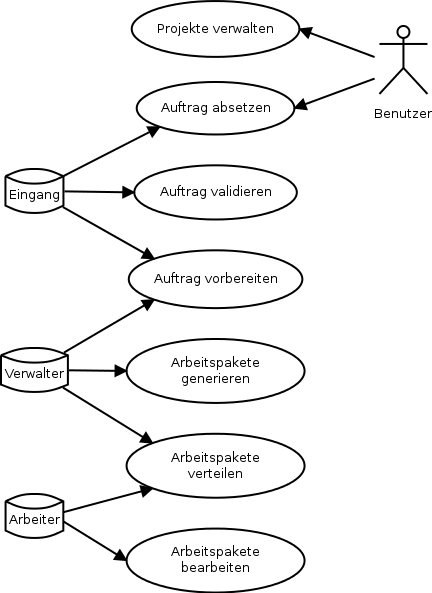
\includegraphics[width=0.7\textwidth]{imageinput/use-case-muss.png}
  \caption{\"Ubersicht Usecases - Kern}
  \label{fig:use-case-muss}
\end{figure}

Wie in \Cref{fig:use-case-muss} gezeigt,
stellt sich der absolute Kern eines CI-Systeme aus relativ wenigen Funktionalitäten zusammen.

Die erste notwendige Funktion stellt die Verwaltung von Projekten \deffeat{projekt-verwalten} dar.
Sind diese dann angelegt, kann man damit beginnen, Aufträge abzusetzen \deffeat{auftrag-absetzen}.
Ist ein Auftrag abgesetzt, so muss seine Richtigkeit sichergestellt werden \deffeat{auftrag-validieren},
danach kann er für die Bearbeitung \deffeat{auftrag-vorbereiten} vorbereitet werden.

Nachdem der Auftrag an sich vorbereitet ist, müssen entsprechend der Build-Matrix \deffeat{auftrag-matrix}
Arbeitspakete generiert werden \deffeat{arbeitspacket-generieren}.
Diese Arbeitspakete werden anschließend verteilt \deffeat{arbeitspacket-verteilen} und abgearbeitet \deffeat{arbeitspacket-abarbeiten}.

Das Abarbeiten der Arbeitspakete sollte in Schritten erfolgen \deffeat{arbeitspackete-schritte},
wobei die grundlegende Art von Arbeitsschritten das Ausführen eines Prozesses \deffeat{arbeitsschritt-prozess} ist.


\subsection{Weiterführende Funktionen}

Nach der Umsetzung des funktionalen Kerns als Basis
k\"onnen nun weiterf\"uhrende Funktionen angelagert werden.
Diese sind nicht zwingend notwendig, tragen jedoch erheblich dazu bei,
informierte Entscheidungen \"uber den Zustand eines Projektes in Integration zu treffen.

\subsubsection{Datensammlung}

Zun\"achst einmal gilt es Datensammlung beim Ablauf eines Arbeitsschritts zu betrachten.
\"Ublicherweise muss zumindest STDOUT/STDERR schon zur Laufzeit festgehalten \deffeat{arbeisschritt-stdio} werden.
Weiterhin besteht  Interesse an statistisch auswertbaren Daten
wie z.B. den Speicherverbrauch \deffeat{arbeitsschritt-stats}.

Nach dem Ausf\"uhren eines Arbeitsschritts fallen interessante Daten an.
Oftmals sorgt zumindest einer der Arbeitsschritte für das Generieren eines ausführbaren Programms.
Dieses sollte sp\"ater auch zur Verf\"ugung gestellt werden \deffeat{arbeitsschritt-artefakt}.
Weiterhin finden sich Test-Resultate in diversen Standardformaten \deffeat{arbeitsschritt-resultate},
wie z.B. JunitXML \cite{jenkins:junitxml} oder \ac{TAP}.

\subsubsection{Arten Arbeitsschritte}

Bei den Arten der Arbeitsschritte gibt es für gew\"ohnlich mehrere M\"oglichkeiten (siehe Kapitel~\ref{chap:ist-analyse}).
Neben den gewohnten Prozess-Schritten (\reffeat{arbeitsschritt-prozess}) sind weitere Arten \"ublich.
Interaktionen mit dem Quellcodemanagement \deffeat{arbeitsschritt-scm} sowie
Schritte implementiert in einer Skript-Sprache \deffeat{arbeitsschritt-script}
stellen weiterf\"uhrende Hilfen dar.

\subsubsection{Verteilung von Arbeitspaketen}

Um \"uberhaupt bis zu den Arbeitsschritten zu kommen,
ist es notwendig, \mbox{Arbeitspakete} zu verteilen \deffeat{arbeitspackete-verteilen}.
Dies soll ein verteilter Prozess sein \deffeat{arbeitspackete-autonome-verteilung},
bei dem die Slaves/Arbeiter aktiv mitwirken k\"onnen.
Eine denkbare Erweiterung w\"are die Möglichkeit, dass Slaves/Arbeiter
die Arbeitspakete mittels kategorischer Filter auswählen \deffeat{arbeitspackete-verteilung-selektiv}.
Beispiele f\"ur diese sind Plattform oder Betriebsumgebung.

\subsubsection{Auftragseingang und Vorbereitung}

%XXX: web hook gosar

Der Auftragseingang kann sich vielseitig gestalten.
Moderne Systeme unterstützen eine Vielzahl von Medien \deffeat{auftrag-eingang-medien},
wie z.B. E-Mail, Web-Hooks, Web-Formulare oder zeitgesteuerte Systeme.

W\"unschenswerte Erweiterungen, welche nicht von existierenden Systemen unterst\"utzt werden,
sind die Anreicherung eines Auftrages um eigene Daten/\"Anderungen.
Besonders hilfreich erscheint hierbei das sogenannte Workdir-diff \deffeat{auftrag-eingang-diff},
welches die aktuellen \"Anderungen eines Entwicklers darstellen.
Dies macht sie besonders n\"utzlich f\"ur den laufenden Entwicklungsprozess.

\subsubsection{Resultatanalyse}

Analyse von Resultaten ist ein vielseitiges Thema,
welches vorwiegend Aufgabe der Erweiterungen sein soll.

In der grundlegend eingebauten Ausf\"uhrung soll zumindest der Erfolg oder Misserfolg
von Auftr\"agen, Arbeitspaketen und Arbeitsschritten feststellbar sein \deffeat{einfache-resultate}.

Die weitergehende Analyse von Ergebnissen soll mittels Erweiterungen behandelt werden.

\subsection{Exemplarische Erweiterungen}

Um die Erweiterbarkeit des Systems aufzuzeigen,
sollen zwei exemplarische Erweiterungen betrachtet werden.
Diese werden hier nur grob umrandet und dann sp\"ater in der Analyse genauer spezifiziert.

Die erste Erweiterung betrachtet vergleichende Analysen von Testergebnissen \deffeat{ext-testing}.
Dabei sollen Entwickler in die Lage versetzt werden,
das Fehlerverhalten eines Programms in verschiedenen Konfigurationen und Auftr\"agen zu vergleichen.
Dies dient zur Vereinfachung der Fehleranalyse.

Die zweite Entwicklung betrachtet ein gänzlich anderes Thema.
Dabei soll das Verhalten einer Version eines Programms
in sehr vielen Kombinationen verst\"andlich gemacht werden \deffeat{ext-analysis}.
Dies soll die Flexibilit\"at des Systems zeigen und
Ideen f\"ur neue Ans\"atze und Werkzeuge bei der Qualit\"atssicherung liefern.


%XXX eventuell spaeter
%\subsection{Vorgaben f. Entwiclungsumgebung}?
%- testen notwendig
%- das system selber ci unterziehen

% %- regeln


\section{Testkriterien}
\label{sec:target:tests}

Dieser Abschnitt beschäftigt sich mit verschiedenen Tests,
die zur Sicherstellung der Funktionalität des Systems notwendig sind.
Dies sind zum einen alle Arten von automatischen Tests,
die auch dazu verwendet werden sollen, das System an sich einer \ac{CI} zu unterziehen
und zum anderen die Manuellen Tests, welche schwer automatisierbare Vorgänge festhalten.


\subsection{Unit-Tests}

Unit-Tests werden verwendet, um die kleinsten Komponenten des Systems zu testen.
Durch ihre starke Koppelung an Implementation und Entwurf
sind sie w\"ahrend der Kriterien-Findung noch nicht n\"aher bestimmbar.

Sie ergeben sich zum Teil im Entwurf und vorwiegend in
der nachfolgenden Implementation.

\subsection{Funktionale Tests}

Funktionale Tests testen einzelne, funktionale Komponenten des Systems.
Daher entsprechen sie grob den funktionalen Anforderungen und Use-Cases.
%XXX: mehr text

\subsection{Systemtests}

Systemtests testen Kombinationen von funktionalen Komponenten sowie das Komplettsystem.
Im Rahmen dieser Arbeit werden drei Systemtests definiert.


\begin{description}
  \item[Komponentendurchlauf:]
    Der Komponentendurchlauf soll anhand des Ausführens der einzelnen, funktionalen Komponenten aufzeigen,
    ob das Zusammenspiel der Komponenten grunds\"atzlich funktioniert.
  \item[Komplettstystem:]
    Der Test des Komplettsystems soll das komplette CI-System auf einer Testdatenbank starten
    und seine Funktion sicherstellen
  \item[Beispiel Datenanalyse:]
    Das Beispiel Datenanalyse soll die Funktion der Beispielerweiterung für die Datenanalyse sicherstellen
\end{description}

\subsection{manuelle Tests}

Die manuellen Tests umfassen alle Tests,
deren Umsetzung als automatisches Programm erfahrungsgemäß zeitaufwendig,
fehleranfällig und/oder umfangreich ist.
Sie werden deshalb von Hand ausgeführt.

\begin{description}
  \item[Zeitliches Verhalten:]
    Die Beobachtung und Analyse des Zeitverhaltens
    bei wachsender Datenmenge und Auftragsgröße soll Aufschluss über algorithmische Engpässe geben.
  \item[Race-Conditions:]
    Die Beobachtung und Analyse trivialer Race-Conditions
    bei wachsender Nebenl\"aufigkeit soll Probleme bei der Skalierbarkeit aufdecken.
  \item[Verhalten bei Systemfehler:]
      Der Verhaltenstest bei Systemfehlern dient der
    \"Uberpr\"ufung des Verhaltens beim Absturz von Teilkomponenten.
  \item[Große Datenanalyse:]
    Die Große Datenanalyse wird die exemplarischen Erweiterungen mit Datenmengen und Aufgaben,
    welche den Rahmen eines automatischen Tests sprengen überprüfen.
\end{description}


\section{Abgrenzung}
\label{sec:target:abgrenzung}

In dieser Arbeit sollen nur der prototypische Kern eins \ac{CI}-Systems
sowie exemplarische Erweiterungen geschaffen werden.
Somit sind viele Themen, welche für ein produktiv eingesetztes \ac{CI}-System notwendig
sind, nicht weiter zu betrachten.
Benutzer und ihre Rechte sollen nicht betrachtet werden.
Authentifikation und Authorisation sind weitreichende Themengebiete,
die sorgfältig betrachtet werden müssen.
Dies ist neben der Hauptaufgabe nicht im zeitlichen Rahmen unterzubringen.
Außerdem wird kein Wert auf die Benutzeroberfläche gelegt.
Intuitive Benutzerinteraktion ist ein überaus umfangreiches Thema.
Dabei sind auch weiterführende Interaktionen,
wie z.B. Konfiguration der Replikation ausgeschlossen.


\section{Zusammenfassung}
\label{sec:target:zusammenfassung}
%XXX: more text

Die wesentliche Aufgabe ist es, den Kern des \ac{CI}-Systems als Protoyp zu schaffen.
Anschließend sollen weitere Funktionen sowie exemplarische Erweiterungen
auf dieser Basis geschaffen werden.
L\"osungskonzepte f\"ur die einzelnen Komponenten sollen vorgestellt werden,
um anschließend ihre Eigenschaften zu betrachten.

Fokus sind dabei die Interaktionen mit der Datenbank und die Datenoperationen.
Semantik des Systems und das Konsistenz-Verhalten bei Datenbankpartitionierung
sollen betrachtet werden. Erweiterungen zur Datenanalyse sollen ebenfalls nur auf technischer Ebene behandelt werden.

Themen wie Benutzerschnittstellen, Rechteverwaltung und Details
von visueller Komponentenintegration werden dabei nicht betrachtet.
Ziel dieser Arbeit ist die Betrachtung der Kernfunktionen und Erweiterungen auf Datenbank-Ebene.

% zusammenfassung 
%   - im wesentlichen soll \ldots. prototypisch & exemplarisch
%   anhand .. soll ein loesungskonz vorgestellt werden

%\chapter{Theoretischer (15\%)}
\section{Problemlösungsansatz}
\section{Modellierung Gundlegender Abfragen}

\chapter{Analyse \& Design ( 25 \%)}
\label{chap:design}

Im vorhergehenden Kapitel wurden Ziele und Leistungskriterium
für das CI-System festgelegt.
Diese sollen nun auf konzeptueller Ebene umgesetzt werden.
Dazu wird zuerst ein Überblick des Gesamtkonzeptes gegeben.
Anschließend werden besondere Konzepte zur 
%XXX: continue


\section{Systemarchitektur}
\label{sec:design:sysarch}
Diese Sektion gibt Aufschluss über die Grobstruktur des CI-Systems auf logischer und physischer Ebene.

\subsection{logisch}

\begin{figure}[ht]
  \centering
  \label{fig:grob-layout-komponenten-logisch}
  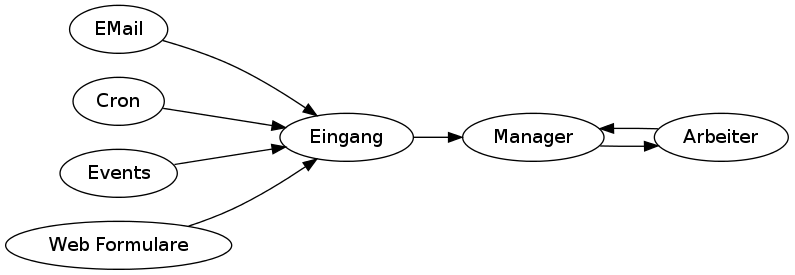
\includegraphics[width=\textwidth]{imageinput/grob-layout-komponenten-logisch.png}
  \caption{\"Ubersicht ber Systemkomponenten - logisch}
\end{figure}


Die erste wichtige Komponente ist der Eingang,
in ihm gehen Aufträge aus verschiedensten Quellen ein.
Nach dem sie validiert wurden, werden die Aufträge an
die zweite wichtige Komponente, den Manager, weitergegeben.
Dort werden sie vorbereitet und entsprechend der Build-Matrix Arbeitspakete erstellt.
Nun treten Manager und Arbeiter in eine Interaktion,
um zu bestimmen welcher Arbeiter das Eigentliche Arbeitspaket bearbeitet.
Anschließend werden die Arbeitspakete von den jeweilig designierten Arbeitern abgefertigt.

%XXX: more


\subsection{physisch}

\begin{figure}[ht] 
  \centering
  \label{fig:grob-layout-komponenten}
  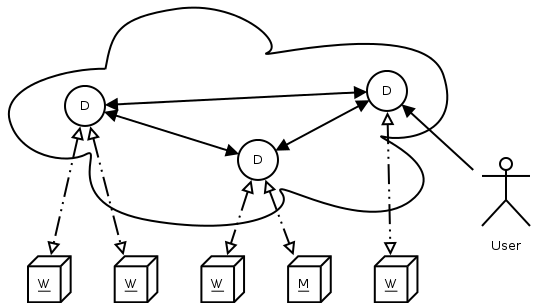
\includegraphics[width=\textwidth]{imageinput/grob-layout-komponenten.png}
  \caption{Übersicht über Systemkomponenten - physisch}
\end{figure}

Der physische Aufbau unterscheidet sich stark von den bisher dagewesenen CI-Systemen.
Grund ist der Fokus auf die verteilte Datenbank, direkte Kommunikation
wird der Interaktion mit einer verteilten Datenbank weichen.

Das System besteht somit aus Komponenten welche alle als Clients einer verteilten Datenbank operieren.
Die Abbildung~\ref{fig:grob-layout-komponenten} zweigt die Struktur.
Nennenswert ist dabei die Bindung einer Komponente and bestimmte Datenbank-knoten,
dies dient der Kontrolle der Lokalität und wird später noch vorgestellte Verfahrensweisen unterstützen.

%XXX more

\section{Datenschema}


\begin{figure}[ht] 
  \centering
  \label{fig:datenstrukturen}
  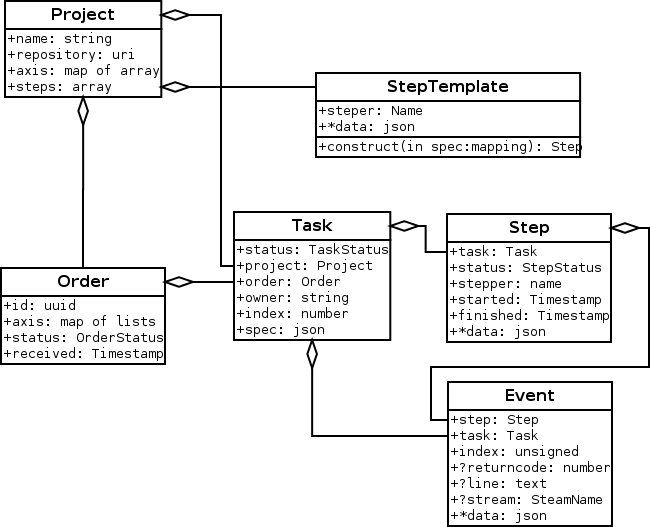
\includegraphics[width=\textwidth]{imageinput/datenstrukturen-step-templates.png}
  \caption{Grundlegende Datenstrukturen}
\end{figure}

Das grundlegende Datenschema, in Abbildung~\ref{fig:datenstrukturen} als UML Klassendiagramm dargestellt,
beschreibt die Daten des Kernsystems und einige ihrer Interaktionen.

Die wichtigsten Datentypen sind dabei Projekt, Auftrag (Order),
Arbeitspaket (Task) und Arbeitsschritt (Step).

\subsubsection{Projekt}

Das Projekt beinhaltet neben dem Namen auch alle Informationen,
die später für das Erstellen von Arbeitspaketen sowie
die Ausführung einer Integration benötigt werden.
Dazu gehört das Quellcode-repository (repo), von dem später
die Quelltexte für das dem Test unterworfenen Projekt bezogen werden.
Weiterhin beinhaltet es die Build-Achsen,
welche die Wertebereiche der einzelnen Ebenen der Build-Matrix
beschreiben.

\subsubsection{Arbeitsschritt Templates}

Der mitunter wichtigste Teil eines Projektes ist jedoch die Beschreibung der Arbeitsschritte als Templates.
Die Darstellung als Template ist dabei bewusst gewählt,
sie ermöglicht es jedem Arbeitspaket speziell konfigurierte Arbeitsschritte zur Verfügung zu stellen.
Außerdem bewirkt die erneute Speicherung in der Datenbank,
das Bearbeiten der Schritte eines Projektes keinen Einfluss auf bereits erstellte Arbeitspakete hat.
Zudem stellen die extra Objekte auch einen Anschlusspunk für die Datensammlung dar.
Die Methode \textit{construct} des Templates dient dazu,
einen Arbeitsschritt, angereichert mit einer entsprechenden Konfiguration, zurückzugeben.

\subsubsection{Auftrag}

Ein Auftrag beinhaltet grundsätzlich eine Referenz auf das zugehörige Projekt,
außerdem beinhaltet er Überschreibungen/Zusätze für die Build-Achsen,
dies Ermöglicht es sowohl in den Achsen eingeschränkte,
als auch erweiterte Aufträge zu erstellen.
Diese werden später genauer erklärt.
Zusätzlich beinhaltet der Auftrag einen Status, dieser beinhaltet den aktuellen Stand der Bearbeitung.

\subsubsection{Arbeitspaket}
%XXX: eventuell projekt hier nicht referenzieren
Ein Arbeitspaket beinhaltet neben Referenzen zu dem Projekt und dem Auftrag,
seine Spezifikation. Diese gibt die Ausbildung aller Build-Achsen für dieses Paket an.
des weiteren beinhaltet es den Index, dieser gibt die Numerische Position in der Build-Matrix an.
Auch ein Arbeitspaket hat einen Status, welcher den aktuellen Bearbeitung-stand zum Ausdruck bringt.
Zudem bestimmt das Feld ``Owner'' den Arbeiter, welcher das Arbeitspaket letztendlich bearbeiten wird.

\subsubsection{Arbeitsschritt}

Ein Arbeitsschritt referenziert das zugehörige Arbeitspaket.
Neben den Zeitpunkten für Anfang und Ende seiner Ausführung,
benennt er im Feld ``stepper'' um welche Art von Arbeitsschritt es sich handelt.
Das Feld ``status'' gibt Auskunft über den aktuellen Stand der Bearbeitung.
Das Feld ``data'' soll weitere dynamische Informationen zum Ausdruck bringen,
die bei der Ausführung genutzt werden.

%XXX: dies dient \ldots


\subsubsection{Event}
%XXX referenz auf task?

Das Event bringt Datensammlung zur Laufzeit zum Ausdruck.
Neben den Referenzen für den Arbeitsschritt und das Arbeitspaket,
beinhaltet es eine Indexnummer und einen Timestamp.
Die Indexnummer ist eine aufsteigende Zahl
und gibt den Events eines bestimmten Arbeitsschritts eine feste eindeutige Reihenfolge.
Der Timestamp gibt den Events eine zeitliche Ordnung (welche jedoch nicht eindeutig ist).


Zusätzlich zu diesen Basisdaten, beinhaltet ein Event beliebige weitere optionale Felder.
Einige mögliche (und ihre Datentypen) sind:

\begin{description}
    \dhitem[returncode: Number] Rückgabe-wert eines Prozesses bei seiner Beendigung.
    \dhitem[line: Text] Textzeile eines Datenstromes der Ausgabe
    \dhitem[lineno: Number] Zugeh. Zeilennummer
    \dhitem[stream: Name] Zugeh. Name des Datenstromes
    \dhitem[start: Name] Mitteilung über den Start eines best. Vorganges
    \dhitem[end: Name] Mitteilung über den Abschluss eines best. Vorganges
\end{description}




\section{Logik der Komponenten}

Diese Sektion behandelt die grundlegende Logik  der Einzelteile des Systems,
sie bilden die Bausteine für das Gesamtsystem.

%XXX MORE

\subsection{Auftragsannahme}

Der Auftragsannahme lässt sich grob in 2 Abschnitte einteilen.
Zuerst geht ein Auftrag ein, was je nach Methode in mehrere Schritte beinhalten kann,
danach wird er überprüft und damit angenommen oder abgelehnt.


\begin{figure}[ht]
  \centering
  \label{fig:lebenszyklus-auftrag-eingang}
  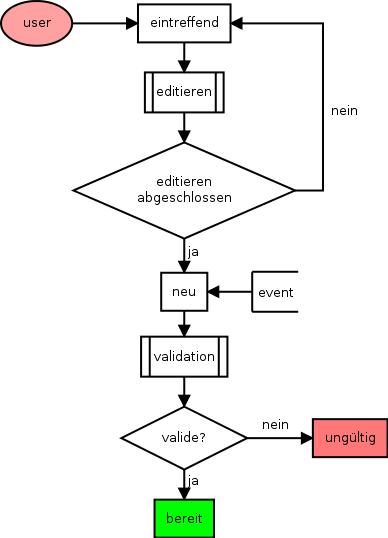
\includegraphics[height=5in]{imageinput/lebenszyklus-auftrag-eingang.png}
  \caption{Auftragsannahme: Flussdiagramm}
\end{figure}


\subsubsection{Eingang}

Auftragseingang gestaltet sich in der Praxis vielseitig.
Da nicht alle Quellen direkt einen fertigen Auftrag generieren können,
beginnt ein Auftrag im Zustand eingehend, sind schließlich alle Daten zusammengekommen,
so wird der Eingang festgehalten und der Auftrag wird vom System weiterverarbeitet.

%XXX Quellen betrachten``
Betrachtet werden die Anforderungen für die Quellen
\begin{description}
    \dhitem[EMail]
        Eingang per EMail kann in 2 Formen erfolgen,
        zum einen kann der gesamte Auftrag ein einer einzigen EMail enthalten sein.
        Zum anderen kann sich der Auftrag über mehr als eine EMail erstrecken.
        Beispiel hierfür sind z.B. Mercurial Patchbombs \cite{mercurial:patchbomb}.
        Ist ein Auftrag fertiggestellt, so ist eine Antwort-email hilfreich.
        Wichtig ist, dass EMails Unbekannter auf keinen Fall
        akzeptiert werden sollten.
    \dhitem[Mailingliste]
        Eingang per Mailingliste ist dem Eingang per Email sehr ähnlich,
        Haupt-unterschied ist, dass anstelle einer privaten Korrespondenz
        ein öffentliches Forum genutzt wird. Dabei sollen auch EMails Unbekannter 
        bearbeitet werden können.
        Ein bekanntes Beispiel für eine Mailingliste mit Patches
        ist die Mercurial Mailingliste \cite{mercurial:mailingliste}.
    \dhitem[Web Formular]
        Web Formulare bieten eine intuitive Möglichkeit,
        einen Auftrag zu bearbeiten und vorzubereiten,
        bevor man ihn letztendlich in Bearbeitung gibt.
    \dhitem[HTTP Hook]
        Http Hooks sind ein Traditionelles Werkzeug,
        um CI-Systemen Änderungen mitzuteilen.
        Sie sind einfach in externe Werkzeuge wie z.b. SCM integrierbar,
        und dienen dazu, Aufträge für die Standardkonfiguration
        eines Projektes abzusetzen, wenn externe Ereignisse,
        wie z.b. ein SCM commit, eintreten.
    \dhitem[Zeitsteuerung]
        Zeitsteuerungen sind ein weiteres Traditionelles Werkzeug,
        um Aufträge in Standardkonfiguration abzusetzen.
        Zu festgesetzten Zeitpunkten, wie z.b. Nachts oder nach
        Arbeitsschluss, werden Aufträge abgesetzt.
    \dhitem[Http API]
        Eine HTTP API kann als Basis sowohl für Testwerkzeuge,
        als auch für WebFormulare dienen.
        Sie ermöglicht Programmen ein hohes maß an Kontrolle
        für das Absetzen von Aufträgen
\end{description}

Fur den Prototypen ist zumindest die ``HTTP API"" notwendig,
um dem System zu Demonstrationszwecken Aufträge zu erteilen.


\subsubsection{Validation}

%XXX: genauer beschreiben

Die Validation verfolgt das Ziel, Aufträge auch aus weniger vertrauenswürdigen Quellen anzunehmen.
Dies ermöglicht Verwendung ähnlich zu TravisCI, was es erlaubt, Zuarbeiten von Außenstehender zu Testen.
Für die Überprüfung stehen verschiedene Möglichkeiten zur Verfügung.
Ein Eingang per Mail/Mailingliste oder Pull-Request auf einer Code-Hosting,
kann z.b. nach erstmaliger Erlaubnis, wiederholt zugelassen werden,
während Informationen die Mitarbeiter einsenden z.b. an ihr Arbeitsverhältnis gebunden werden können.

Zeitgesteuerte Eingänge innerhalb des Systems können jedoch grundsätzlich zugelassen werden.

Den Abschluss der Validation stellt die Markierung des Auftrages als Valide oder invalide dar.

\subsection{Management}

\begin{figure}[ht] 
  \centering
  \label{fig:lebenszyklus-auftrag-abarbeitung}
  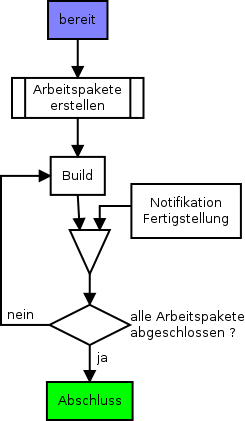
\includegraphics[height=4in]{imageinput/lebenszyklus-auftrag-abarbeitung.png}
  \caption{Auftragsannahme: Flussdiagramm}
\end{figure}

\subsubsection{Auftragsvorbereitung}

In der Auftragsvorbereitung werden Details aus dem Projekt zum Auftrag hinzugefügt.
Die vordefinierten Build-Achsen werden vom Projekt übertragen.
Dies stell sicher, dass der Aufrag und sein Umfang eindeutig bestimmt sind,
bevor mit der Erstellung von Arbeitspaketen begonnen wird.


\subsubsection{Bereitstellung von Arbeitspaketen}

Das Bereitstellen von Arbeitspaketen stellt den Anfang der eigentliche Arbeitsphase dar.
Entsprechend der Werte der Build-Achsen des Auftrages, werden nun die Arbeitspakete generiert,
wobei jedes Arbeitspaket eine der Wertekombinationen darstellt.
Nachdem alle Arbeitspakete erstellt sind, ist die Bearbeitung des Auftrages an sich abgeschlossen.

\subsubsection{Abschluss von Aufträgen}

Der Abschluss eines Auftrages ist ein Ereignis, welches Impliziert werden kann.
In im zu entwickelnden System wird der Abschluss eines Auftrages definiert,
als der Zustand der Eintritt, wenn alle Arbeitspakete eines Auftrages
einen finalen Zustand erreichen.

Dies Vereinfacht die Behandlung des Auftragsabschlusses,
da man nicht nach Abschluss von Arbeitspaketen weitere Operationen durchführen muss,
um den eventuellen Abschluss festzustellen.

\subsection{Zuteilung/Abarbeitung von Arbeitspaketen}


\subsubsection{Lebenszyklus eines Arbeitspaketes}


\begin{figure}[ht] 
  \centering
  \label{fig:lebenszyklus-arbeitspaket}
  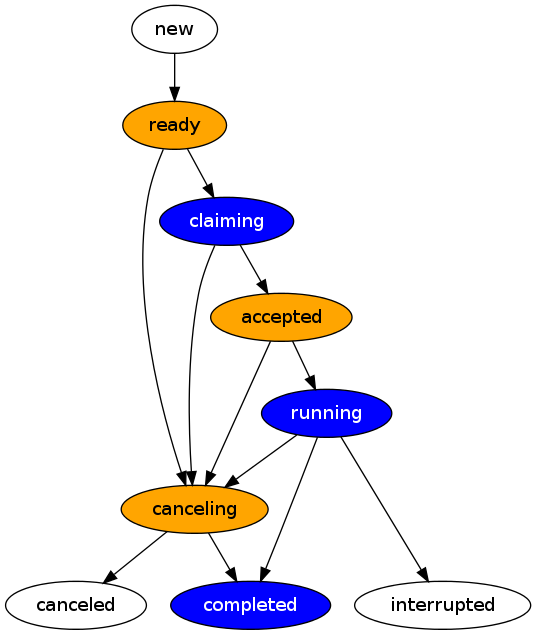
\includegraphics[height=4.5in]{imageinput/lebenszyklus-arbeitspaket.png}
  \caption{Lebenszyklus eines Arbeitspaketes bei Ausschreibungen}
\end{figure}


\subsubsection{Vorbereitung Abarbeitung}

\subsubsection{Zuteilung}


\subsubsection{Abschluss Abarbeitung}

Ist die Bearbeitung der einzelnen Schritte eines Arbeitspaketes abgeschlossen,
so muss das Resultat zusammen

- ende der arbeisschritte
- zusammenfassung resultat
- endscheidung fehlschlag oder nucht


\subsection{Überblick Methoden der Zuteilung von Arbeitspaketen}

Diese Sektion beschäftigt sich mit der Zuteilung von Arbeitspaketen.
Grundsätzlich gibt es 2 Möglichkeiten dies zu bewerkstelligen.
Es muss festgestellt werden, welche Methode besser geeignet ist.

\subsubsection{Melde-verfahren}
% MOAR
Beim Melde-verfahren teilt der Arbeiter nur seinen Arbeitwunsch mit.
Anschließend wartet er darauf, dass dieser Erfüllt wird.
Dabei liegt die Logik der Zuteilung komplett beim Manager,
er muss also über das Wissen verfügen, welcher Arbeiter in der Lage ist welche Arbeitspakete zu bearbeiten.

\begin{figure}[ht] 
  \label{fig:auftrag-zuteilung-token}
  \begin{sequencediagram}
      \newinst{worker}{:Worker}
      \newinst[1]{manager}{:Manager}
      \mess{worker}{token <spec>}{manager}
      \mess{manager}{work <spec>}{worker}
      \mess{worker}{result}{manager}
  \end{sequencediagram}
  \caption{Auftragszuteilung: Tokenbasiert}
\end{figure}

Vorteil des Verfahrens ist, das die Zuteilung ein eindeutiger Prozess ist.
Jedoch benötigt der Manager genaues wissen über die Arbeiter,
um seiner Aufgabe gerecht zu werden.

\subsubsection{Ausschreibungsverfahren}

Beim Ausschreibe-verfahren teilt der Manager die offenen Arbeitspakete mit.
Anschließend können Arbeiter einen Anspruch auf diese Anmelden.
Sie treten dabei in Konkurrenz.
Der Manager entscheidet dann, welcher Arbeiter welches Arbeitspaket bearbeiten darf.
%MOAR

Dies erlaubt Wesentlich autonomere Arbeiter,
sie sind nun in der Lage frei zu entscheiden,
welche der verfügbaren Aufträge sie bearbeiten wollen.
Der Manager ist auch Vereinfacht,
da er nur noch die Entscheidung für den Zuschlag treffen muss.
es ist nicht notwendig spezielles Wissen über die Arbeiter zu haben. 


\begin{figure}[ht] 
  \label{fig:auftrag-zuteilung-claim}
  \begin{sequencediagram}
      \newinst{workera}{:Worker A}
      \newinst[1]{manager}{:Manager}
      \newinst[1]{workerb}{:Worker B}
      \mess[1]{manager}{availiable}{workera}
      \prelevel
      \prelevel
      \mess[1]{manager}{availiable}{workerb}

      \mess[1]{workera}{claim}{manager}
      \prelevel
      \prelevel
      \mess[2]{workerb}{claim}{manager}
      %XXX: better call?
      %\prelevel
      %\prelevel
      %\begin{call}{manager}{approve}{manager}{workera}
      %\end{call}
      \mess{manager}{approve A}{workera}
      \prelevel
      \mess{manager}{approve A}{workerb}
  \end{sequencediagram}
  \caption{Auftragszuteilung: Ausschreibungsbasiert}
\end{figure}

\subsubsection{Auswahl}

Das Ausschreibungsverfahren zeigt sich im Vergleich zum Melde-verfahren
wesentlich flexibler.
Die Möglichkeit Detailkenntnisse über die Fähigkeiten eines Arbeiter nur
beim Arbeiter zu belassen, sorgt dafür, das Arbeiter wesentlich autonomer sind.
Dies hat zur Folge, dass der Zuteilungs-algorithmus wesentlich vereinfacht wird.
Da für ihn nun unerheblich ist, er den Zuschlag bekommt.
Das Ergebnis wird das gleiche sein.

\subsection{Abarbeitung von Arbeitspaketen}

Bei der Abarbeitung von Arbeitspaketen geht es darum die einzelnen Arbeitsschritte
der reihe nach linear abzuarbeiten.
es 

\subsubsection{Arbeitsschritte}


\begin{figure}[ht] 
  \centering
  \label{fig:lebenszyklus-arbeitsschritt}
  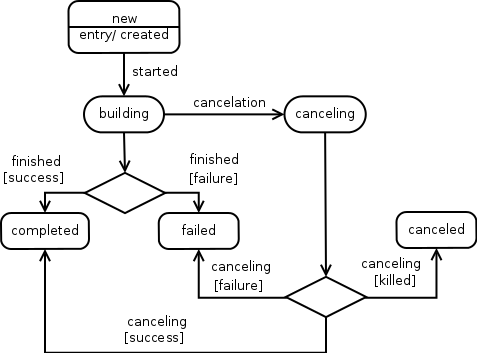
\includegraphics[height=3.4in]{imageinput/lebenszyklus-arbeitsschritt.png}
  \caption{Stategraph eines Arbeitschrittes}
\end{figure}

\begin{verbatim}
- kill wird in der impl nicht betrachtet

\end{verbatim}


\subsubsection{Datensammlung zur Laufzeit}

\begin{verbatim}
- sinn/echtzeit?

- beispielhaft
    - STDOUT/ERR
    - exakte testresultate/reports
\end{verbatim}



\subsubsection{Datensammlung nach Abschluss eines Schrittes}

Datensammlung nach dem Abschluss eines Arbeitsschritts,
Umfasst in der Regel verschiedenste Dateiformate.
Diese werden aus den verschiedensten Gründen generiert.
Üblich sind Test-Resultate, Logdateien, Build-Resultate und Archive.

Die Abbildung dieser Datensammlung kann dabei auf 2 Arten geschehen,

\begin{enumerate}
    \item als Teil des Schrittes
    \item als eigene Art von Schritt
\end{enumerate}

Die Abbildung als eigene Art von Arbeitsschritt,
hat einige Vorteile, da sie die Zuständigkeit vom reinen Arbeitsschritt
und dem Daten-sammeln sauber trennt.

Dies macht die Werkzeuge zur Datensammlung wesentlich einfacher.
Anstatt sie in jeden Schritt integrieren zu müssen,
kann einfach nach dem Schritt angewendet werden.


\subsubsection{Abschluss von Arbeitsschritten}

- returncodes
- fehler

\section{Besondere Ansätze zur Datenbank-Interaktion}

%XXX: http://dbmsmusings.blogspot.de/2010/04/problems-with-cap-and-yahoos-little.html


\subsection{CAP Abdeckung}

Wie bereits in Sektion~\ref{sec:base:cap} erwähnt,
ist es immer nur möglich 2 der 3 Aspekte des CAP Theorems abzudecken.

Jedoch ist es durchaus legitim für verschiedene Teile
einer verteilten Applikation unterschiedliche Bereiche abzudecken.
Sobald genau definiert ist, für welche Daten in welchem Kontext welche Eigenschaften benötigt werden,
kann ein konsistentes Modell geschaffen werden.

Wichtig ist bei dieser Betrachtung, dass die unterschiedlichen Komponenten des Entwickelten CI-Systems
nicht zwingend eine direkte Konsistenz-Bindung untereinander benötigen.
Wichtig ist nur, die Konsistenz zwischen einer Komponente
und dem Datenbank-knoten, mit dem sie Kommuniziert.

Das Haupt-system, in dem alle Komponenten in Kommunikation stehen,
%XXX: s1?
soll nach Systemanforderung \textbf{S1} immer verfügbar sein und somit einen Teil-Ausfall  verkraften.
Somit kommt für die Kommunikation zwischen Komponenten nur das Modell \textbf{A-P} in Frage
(was Verfügbar und Partitionstolerant bedeutet).

Die Anbindung einzelner Komponenten and ihre Datenbank-knoten, hat jedoch andere Anforderungen.
Da eine direkte Anbindung and die Datenbank für das Funktionieren einer Komponente unabdingbar ist,
kann in diesem Fall nur das Modell \textbf{C-A} zum Einsatz kommen.


%XXX: http://www.infoq.com/articles/cap-twelve-years-later-how-the-rules-have-changed


\subsection{Status-Maschinen zur Wahrung der Konsistenz}

%XXX: Literatur
% http://blog.incubaid.com/2012/10/25/caulking-your-distributed-algorithm-implementation/
\nocite{statechart}

Statusmaschienen sind ein allgemein bekanntes Werkzeug,
um den den Ablauf eines komplexen Programms zu beschreiben oder zu erklären.
In der Regel wird dazu ein sog. StatusGraph verwendet.
Dieser ist ein Gerichteter Graph der die Zustände und Zustandsänderungen eines Systems beschreibt.

Wie bereits in Abbildung \ref{fig:lebenszyklus-arbeitspaket} gezeigt,
stellt der Lebenszyklus eines Arbeitspaketes einen solchen Statusgraph dar.
Als Besonderheit ist er sogar frei von Zyklen.
Dadurch ist es unmöglich den gleichen Status noch einmal zu erreichen.

Bindet man Zusätzlich noch die Transitionen an bearbeitende Knoten (Agenten außerhalb der Datenbank),
so ist es auch bei einer Partitionierung der Datenbank eine Konsistenz der Gesamtsystems gewährleistet.

%XXX: moar?


Mit dem dem Eingang und der Abarbeitung von Aufträgen verhält es sich ähnlich,
jedoch ist der Graph dort Wesentlich einfacher.
Die Abbildungen \ref{fig:lebenszyklus-auftrag-eingang} und \ref{fig:lebenszyklus-auftrag-abarbeitung} zeigen den groben Ablauf.
Der Wechselpunkt zwischen Eingang und Abarbeitung ist die der Validation angeschlossene Markierung zur Bereitschaft.
Da es nur diesen einen Punkt des Austausches gibt, ist die Wahrung der Konsistenz des Auftrages denkbar einfach,
Mit der Bereitschaft, wird die Verantwortung vom Eingang zur Abarbeitung übertragen.

\subsection{Abbildung des Verteilten Systems auf Datenbanken}

Die Abbildung eines verteilten Systems auf eine Datenbank,
hat einige überaus erfreuliche Nebeneffekte.

Im Client-Server System müssen der Client und Server extra Nachrichten Austauschen, um das gleiche Bild der Welt zu bekommen, wobei jedes System eine eigene Version des Zustandes hat.
Beim Datenbank-basierten System ist der Status jedoch in der Datenbank und
die einzelnen Komponenten des Systems müssen somit nicht weiter eigene Kopien vorhalten.

Eine Änderung des Status wird nun durch eine Änderung in der Datenbank zum Ausdruck gebracht.
Sobald die Änderung in die Datenbank eingebracht ist,
ist der Vorgang des Übermittelns für die sendende Komponente abgeschlossen.
Sie muss nicht wie bisher auf eine Rückantwort warten.

\subsection{Auftragsverteilung}

\section{Logisches Gesamtkonzept}
\subsection{Eingang}
\subsection{Management}
\subsection{Arbeiter}

\section{Arbeitsschritte und der Kontext ihrer Ausführung}

\subsection{Überblick und grundlegender Ablauf}

\begin{figure}[!ht]
  \centering
  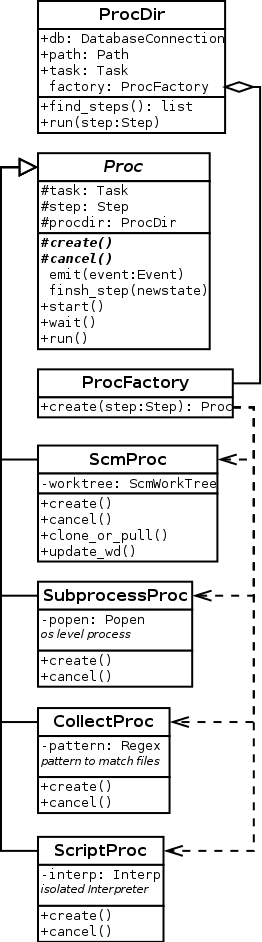
\includegraphics[height=0.8\textheight]{imageinput/klassen-arten-arbeitsschritt.png}
  \caption{Arten und Ablauf von Arbeitsschritten}
  \label{fig:klassen-arten-arbeitsschritt}
\end{figure}

Wie man auf der Grafik~\ref{fig:klassen-arten-arbeitsschritt} gut erkennen kann,
bildet das Arbeitsverzeichniss (ProcDir) die Basis
für die Durchführung der Arbeitsschritte eines Auftrages.

Es bindet alle Operationen, die notwendig sind,
um die Kontrolldaten (Steps, siehe Fig~\ref{fig:datenstrukturen})
aus der Datenbank zu laden und diese dann an Ausführende Objekte zu binden (Proc).

Der Lebenszyklus eines ``Proc'' Objektes wird dabei vom zugehörigen Procdir verwaltet.
das Proc Objekt sollte nur innerhalb der Methode run existieren.
\lstset{language=python}
\begin{lstlisting}
#pseudocode
class ProcDir:
    def __init__(self, procmaker):
        self.procmaker = procmaker
    def run(self, step):
        proc = self.procmaker.create(step)
        return proc.run()
\end{lstlisting}

%XXX: More

\subsection{Prozess Schritte}

Die Aufgabe eines Prozessschrittes ist es,
einen Programm mit vorgegebenen Parametern auszuführen.
Dies ist auch der Grund, warum der ``ProcessProc'' Datentyp einen
Prozess-Handle enthält.

Dabei Fallen zur Laufzeit sammelbare Daten wie z.B. Text auf den Standard Eingabe-/Ausgabe Datenströmen an.
Außerdem verändern sich statistische Informationen über den Prozess wie Speicher-verbrauch, IO-Last, u.a.


\subsection{Skript Schritte}

Skript-Schritte unterscheiden sich von Prozess-Schritten in der Hinsicht,
dass sie kein Programm an sich, sondern ein Skript ausführen.
Daher können sie in die Lage versetzt werden,
weitere Laufzeit-Daten zur Verfügung zu stellen


\subsection{Quellcode Management Schritte}

Quellcode Management Schritte behandeln die Interaktion mit dem SCM.
Es wird, wenn notwendig ein Arbeitsverzeichniss erstellt.
Danach gibt es mehrere Grundlegende Operationen, die durchgeführt werden können.

\begin{description}
    \dhitem[Eingang von Historie]
        bringt die lokale Historie auf den aktuellen Stand, ``pull'' genannt
    \dhitem[Aktualisierung des Arbeitsverzeichniss]
        aktualisiert die Dateien im Arbeitsverzeichniss
        auf eine gewünschte Version
    \dhitem[Anwendung von Patches]
        wendet Patches auf das aktuelle Arbeitsverzeichniss an
\end{description}


\subsection{Datensammlungs Schritte}

Datensammlung-schritte haben die Aufgabe,
bei vorhergehenden Schritten entstandene Dateien 
in die Datenbank zu überführen.
Die Grundfunktion pflegt dabei nur den Inhalt der Datei ein.
Laufzeit-Daten dieses Schritts sind die gefundenen Dateien.

Dabei wird das Regexmuster ``pattern'' verwendet, um festzustellen,
ob eine Datei im Arbeitsverzeichniss, zur Menge der gewünschten Dateien gehört.

Erweiterte Versionen dieser Schritt-Art, könnten zusätzliche Funktionen,
wie z.b. Einpflegen von Testergebnissen aus JunitXML Dateien in die Datenbank,
übernehmen

\section{Erweiterungen}

\subsection{Analyse Test-Resultate}

Bei der Analyse von Test-Resultaten ist das Ziel Veränderungen in Verschiedenen Umgebungen feststellen zu können.
Ziel ist es dabei Vorwiegend Unterschiede zwischen verschiedenen Arbeitspaketen und Aufträgen festzustellen. Unterschiede zwischen Zeitlich aufeinander Folgenden Aufträgen oder Arbeitspaketen, welche verschiedene Plattformen, Entwickler-zweige oder Konfigurationen betrachten, geben Aufschluss über Entwicklung und Zustand des Projektes.

Da ein großer Teil dieser Erweiterung zur Benutzeroberfläche gehört,
werden hier nur die unterstützenden Algorithmen und Datenstrukturen betrachtet.
Um überhaupt Vergleiche anstellen zu können, muss zuerst die Vergleichs-menge bestimmt werden. Dabei erscheint die Menge an Test-Resultaten je Arbeitsschritt am geeignetsten. Im Gegensatz zur Menge an Test-Resultaten je Auftrag,
ist in diesem Fall für jede Konfiguration ein Set an Resultaten verfügbar.

Um Testresultate abzulegen, erscheint es sinnvoll eine weitere Art an Datenstruktur einzuführen.
Diese sollte wie die Bereits definierten ``Events'' aufgebaut sein,
jedoch soll es möglich sein, diese aus einem Prozess der den Testvorgang verwaltet,
anzulegen. Zudem sollen sie an das Arbeitspaket und nicht an den Arbeitsschritt gebunden sein.

Für die Vergleiche ist es nun Notwendig,
Unterschiede zwischen 2 oder mehr Mengen an Testresultaten zu bestimmen.
Eine recht einfache Methode ist dabei die Mengen-Differenz,
Nimmt man für die Testresultate eine Werte-menge mit der Struktur \{ $Testname \rightarrow Resultat$ \} als Basis,
so ist es leicht einen passenden Überblick aufzubauen.

Die Datenstruktur der Resultate, für Vergleiche zischen N Resultatmengen
ist dabei eine Zuordnung von
$\{ Testname \rightarrow ( Resultat_{1},\ldots,Resultat_{N})\}$
Wobei idr. nur die Elemente interessant sind,
deren Resultat-menge Unterschiede und/oder Fehlschläge aufweist.
Ein gutes Beispiel für die Darstellung eines solchen Resultates
stellt der Testresultatüberblick des Pypy Projektes \cite{pypy:overview} dar.

Die Art und Weise wie die Mengen an Test-resultaten für die Vergleiche ausgewählt werden sollen, werden in dieser Arbeit nicht betrachtet,
da dies vorwiegend ein Problem der Benutzeroberfläche ist.

\subsection{Analyse Verhalten eines Programms}

Bei der Erweiterung zur Analyse des Verhaltens eines Programms,
geht es darum das Verhalten eines Programms
in verschiedenen Konfigurationen zu testen.
Als Programm wurde dabei ein Skript gewählt,
welches einen genetischen Algorithmus umsetzt.

Im willkürlich gewählten Beispiel ist dies ein Programm,
welches versuchen soll, eine Funktion anzunähern \cite{gen:prog}.

Die Analyse soll dazu dienen, Parameter-werte festzustellen,
die zum Erfolg des Algorithmus führen.
Bei der Betrachtung steht die Analyse der Resultate nach der Durchführung des Programms im Vordergrund,

Dabei wurden die folgenden Konfigurations-achsen für Parameter gewählt.

\begin{description}
    \item[generations] Menge der Generationen
    \item[population] Größe der Population
    \item[height-weight] Bewertungsgewicht für die Höhe des Baumes welcher die angenäherte Funktion zum Ausdruck bringt
\end{description}

Die Achsen ``generations'' und ``population'' sind dabei ein exponentiell wachsender Wertebereich zwischen 20 und 5000.
Die Achse ``height-weight'' hingegen wurde im Bereich zwischen -2 und 2 gewählt,
wobei viele Werte im Bereich $ 0<abs(x)<1$ liegen.

Die Wahl der Achsen und ihrer Parameter ist willkürlich als Teil eines ersten Tests entstanden.
Weitere Parameter und Achsenkonfigurationen sind denkbar.
Das Analysewerkzeug soll zeigen welchen Einfluss die Parameter haben.

Um dies zu zeigen, ist es notwendig die Resultate
eines Konfigurierten Durchlaufes (Auftrag) Zusammenzufassen.
Die Resultate jedes einzelnen Auftrages sind dabei aus der Standardausgabe
des Programms zu entnehmen.

Für jedes Arbeitspaket eines Auftrages sind also Parameter-werte und Ergebnis zusammenzufassen.
Anschließend können die Daten in Graphen dargestellt werden.


\section{Benutzeroberfläche}

Da die Benutzeroberfläche für den Prototypen nicht zwingend notwendig,
wird darauf verzichtet, mehr als nur simple Werkzeuge zur Verfügung zu stellen.
Wichtig ist dabei, dass vorgefertigte Testdaten in die Datenbank eingegeben werden können.


\section{Zusammenfassung}

was kommt
was kommt nicht

\chapter{Technologische Konzeption}
\label{cha:tech}

Im vorhergehenden Kapitel wurde das grundlegende System konzipiert.
Fortsetzend daran sollen nun geeignete Technologien und Werkzeuge gefunden werden,
um einen Prototyp umzusetzen.
Außerdem sollen notwendige Anpassungen der Konzepte an technische Gegebenheiten vorgenommen werden,
um die fortf\"uhrende Implementation zu unterst\"utzen.


% begruendet technologie, ist trasnformation notwendig

% evtl kap 7 referenzieren


\section{Datenbank}
\label{sec:tech:db}

Die Auswahl der Datenbanktechnologie und eines darauf basierenden Datenbankproduktes sind die wichtigsten technologischen Entscheidungen dieser Arbeit.
Die im \Cref{chap:design} vorgestellten Lösungen sollen als prototypisches System umgesetzt werden.
Die Datenbank stellt die Basis dieses Systems und ihre Eigenschaften werden die Implementation maßgeblich beeinflussen.


\subsection{Technologische Betrachtung}

In einer initialen Sondierung zeigte sich,
dass drei Klassen an Datenbanken die grundlegenden Anforderungen an die Modellierung des Denkschemata erfüllen.
Diese sind die dokumentorientierten Datenbanken, die Graphen-Datenbanken und moderne relationale Datenbanken. 
Eine erklärende Abbildung findet sich in \Cref{fig:klassen-datenbanken}.

\subsection{Produktanforderungen}

Wie die technologische Betrachtung zeigt,
sind mehrere Arten von Datenbank für die Modellierung geeignet.

Um ein geeignetes Produkt zu bestimmen,
m\"ussen Anforderungen herausgearbeitet werden,
welche sp\"ater bei der Implementation hilfreich sein k\"onnten.

Wichtigstes Kriterium ist dabei, dass die Datenbank tats\"achlich \textbf{verteilt} ist.
Um sicherzustellen, das alle Systemanforderungen erf\"ullt werden k\"onnen,
muss die Datenbank zus\"atzlich \textbf{Master-Master-Replikation} beherrschen.
Selbstverst\"andlich muss die Replikation mit einer \textbf{Partitionierung} des Netzwerkes zurechtkommen.

Ein weiteres wichtiges Werkzeug, welches die Datenbank mitbringen sollte, sind \textbf{Mitteilungen über Änderungen}.
Unterschiedliche Komponenten des Systems beginnen mit ihren Aufgaben,
wenn Änderungen an der Datenbank stattfinden.
Daher sind detaillierte Echtzeit-Informationen über Änderungen der Datenbank eine entscheidende Komponente,
deren Einfluss auf Latenzen und Antwortzeiten der Komponenten nicht zu unterschätzen ist.

\subsection{Ausblick}

Die vorgestellten Kriterien lassen noch keine Auswahl des Produktes zu.
Daher wird an dieser Stelle darauf verzichtet, dass Datenschema auf die zur Verfügung stehenden Datenbankarten abzubilden.

\section{Programmiersprachen}
\label{sec:tech:proglang}

Die Programmiersprachen stellen die Basis f\"ur eine produktive Entwicklung,
sie erm\"oglichen erst die Umsetzung eines Projektes.

\subsection{Technologische Betrachtung}

Da ein Prototyp geschaffen werden soll,
ist eine Programmiersprache mit hoher Produktivit\"at gefragt,
selbst wenn dies auf Kosten von Performance geschieht.

Daher bietet sich die Klasse der Skriptsprachen an,
ihre dynamische Natur ermöglicht es,
in kleineren Projekten schnell zum Ziel zu kommen.
%XXX cite?
Weiterhin muss eventuell die Datenbank-interne Sprache beachtet werden.

% klassen/moduldiagramme aus kap 5 referenzieren

\subsection{Produktanforderungen}

Im Detail sind nur einige wenige Punkte zu beachten.
Die Wahl der Sprache an sich steht frei,
solange bestimmte Bibliotheken verf\"ugbar sind.

Wichtig sind dabei vor allem folgende Punkte:
\begin{itemize}
    \item Datenbankzugriff,
    \item Prozesskontrolle für Prozess basierte Arbeitsschritte,
    \item Zugriff SCM und
    \item Automatisches Testen.
\end{itemize}

Außerdem sollte der Entwickler bereits mit der Sprache vertraut sein.
Für die Datenbank-interne Sprache muss sich nach der Datenbank gerichtet werden.


\section{Weitere Werkzeuge}
\label{sec:tech:tools}

Hier werden weitere Werkzeug-Arten und Technologien vorgestellt,
welche die Implementation unterstützen.

\subsection{Testwerkzeuge}

Um die noch zu entwickelnden Unit-Tests,
sowie die bereits in \cref{chap:target} spezifizierten Tests umzusetzen,
ist es notwendig, Tests zu schreiben. Um diese Aufgabe zu erleichtern
sollen Werkzeuge und Frameworks herangezogen werden,
welche die Arbeitsprozesse rund um die verschiedenen Arten von Tests unterstützen.

\subsection{Datenbank Management}

Zur Verwaltung der Datenbank, sowie datenbankinterner Programmteile,
werden Werkzeuge zum Analysieren und Verwalten benötigt.


\section{Konzeptuelle Abbildungen}
\label{sec:tech:konzeptabbildung}

Dieser Abschnitt behandelt konzeptuelle Abbildungen der Ideen aus dem Grobkonzept.
Sie sollen den verwendeten Technologien angepasst werden.

\subsection{Ausschreibungsverfahren für die Auftragserteilung}
\label{sec:verfahren:erteilung}

Für die Umsetzung des Ausschreibungsverfahren der Auftragserteilung gibt es
mehrere Möglichkeiten die Inanspruchnahme eines Auftrages in
der Datenbank umzusetzen. Je nach Fähigkeiten der Datenbank kann man 
alternative Versionen eines bestimmten Datenobjekts nutzen
oder auf separate Datenobjekte, welche die Inanspruchnahme ausdrücken, setzen.

\subsubsection{Alternative Versionen}

Bei der Umsetzung mit alternativen Versionen wird die Technik \ac{MVCC} eingesetzt.
Sinnhaft überbesetzt, bedeutet das Kontrolle der Nebenläufigkeit durch multiple Versionen.

Im Prozess der Zuteilung sind dabei mehrere Versionen eines Arbeitspaket-Objektes vorhanden und jede Version bringt eine andere Inanspruchnahme zum Ausdruck.

Die eigentliche Zuteilung wird anschließend diesen Konflikt wieder bereinigen.
Dabei wird eine neue Version des Arbeitspaketes erstellt, welche den Gewinner festlegt und alle anderen ersetzt.
% More?

\subsubsection{Separate Datenobjekte}

Bei der Abbildung als separate Objekte in der Datenbank
wird für jeden Arbeiter, der ein Arbeitspaket ausführen will, ein $Claim (Paket, Arbeiter)$ erzeugt. Diese bringen Inanspruchnahme zum Ausdruck.
Der Manager kann dann eines dieser $Claim$-Objekte auswählen und dem Arbeitspaket einen Arbeiter zuteilen.
%MORE!

\subsection{Alternativen zu Fabriken in Skript-Sprachen}

Das Fabrik-Muster kommt vorwiegend in statisch-typisierten objektorientierten Sprachen zum Einsatz. In dynamisch typisierten Sprachen gibt es jedoch eine weitere Methode, dass dynamische Instantiieren von abgeleiteten Klassen zu behandeln.

Anstelle einer Fabrik-Klasse, die konfiguriert wird,
kann eine einfache Zuordnung an Konstruktoren anlegt werden.

Dies trifft besonders auf die ``Proc''-Klassen (siehe \Cref{fig:klassen-arten-arbeitsschritt}) zu.
Ihre Zuordnung zu Arbeitsschritten findet über den Wert eines Attributes statt,
daher ist eine eindeutige Zuordnung über ein Mapping ausreichend (siehe \cref{fig:fabrik-mapping}).


\chapter{Implementation}

Dieses Kapitel beschreibt die Implementation des Systems.
Dabei wird zuerst auf Wahl der Werkzeuge eingegangen,
anschließend wird die Struktur beschrieben.
Danach werden Primitiven vorgestellt, welche die Implementation der Komponenten vereinfachen.
Schließlich werden Besonderheiten bei der Implementation einiger Komponenten vorgestellt.
Zum Schluss werden die exemplarischen Erweiterungen vorgestellt.

\section{Werkzeuge}
\subsection{Datenbank}

Das Kriterium der \textbf{Master-Master-Replikation}
schränkt die Auswahl der verwendbaren Datenbanksysteme bereits stark ein.

In die nähere Betrachtung kommen CouchDB \cite{couchdb:website} (dokumentorientiert)
und PostgreSQL \cite{postgresql:website} (relational).
Beide Systeme besitzen Werkzeuge für Master-Master-Replikation
und Primitiven für die Mitteilung von Änderungen.

Andere Systeme wie Mysql (relational) \cite{mysql:website}, Mongodb (dokumentorientiert) \cite{mongodb:website}
und  Neo4J (graph) \cite{neo4j:website} scheiden aus, weil zu ihrem Funktionsumfang
nur die Master-Slave-Replikation geh\"ort.
Das System Riak \cite{riak:website} wurde verworfen, da es Mitteilungen über Änderungen nicht unterstützte und in einem kurzen Vergleich
die Anfragen langsamer beantwortete.

Im oberflächlichen Vergleich von PostgreSQL mit CouchDB ging CouchDB als Sieger hervor.
Im Test mussten bei CouchDB zwar Abstriche im Bereich Performance gemacht werden,
jedoch stellte sich heraus, dass die Mitteilungen über Änderungen von CouchDB detaillierter sind.
Außerdem erscheint der Prozess der Replikation in CouchDB als fehlertoleranter und einfacher, da er fest integriert ist und für asynchrone Replikation mit langen Unterbrechungen konzipiert ist.

In PostgreSQL sind Mitteilungen über Änderungen ein separates Konzept \cite{postgresql:notify}.
Sie sind unabhängig von Änderungen der Datenbank und müssen manuell integriert werden. 
In CouchDB sind Mitteilungen \cite[Chap Notifications]{couchdb:guide} über Änderungen genaue Informationen
über das geänderte Objekt, eventuelle Konflikte der Datenbank
und auf Wunsch sogar das Objekt selbst. Somit erfüllen die Mitteilungen in CouchDB bereits alle Anforderungen.

Somit wurde aufgrund der technischen Vorteile das System CouchDB als zugrunde liegende Datenbank ausgewählt.

\subsection{Programmiersprachen}

Es wurden zwei Programmiersprachen ausgew\"ahlt:
zum Einen Python wegen seiner Bibliotheken und
zum Anderen Javascript, da es die datenbankinterne Sprache von CouchDB ist.

\begin{table}[ht]
\centering
\begin{tabular}{l|c|c}
                            & \textbf{Python} & \textbf{Javascript} \\
    \hline
    datenbankintern         & nein            & ja \\
    Prozesskontrolle        & integriert      & extern, rudimentär \\
    SCM API                & verfügbar       & nicht verfügbar \\
    CouchDB Client          & verfügbar       & verfügbar \\
\end{tabular}
\caption{Überblick über Features und Bibliotheken der Sprachen}
\label{tab:python-vs-js}
\end{table}

Ein besonderes Problem mit Javascript ist,
dass es innerhalb der Datenbank die Bibliotheken, welche datenbankextern sind,
nicht oder nur in limitierter Form verwenden kann.
Die Laufzeitumgebung weist große Unterschiede
zwischen Datenbank-interner und Datenbank-externer Verwendung auf.

Weiterhin konnten wie in \Cref{tab:python-vs-js} aufgezeigt,
für einige benötigte Bibliotheken keine
oder nur unzureichende Implementationen gefunden werden.
Somit ist Javascript für die Implementation der Komponenten
nur sehr bedingt geeignet.

Python hingegen hat Bibliotheken für alle notwendigen Grundfunktionen
und hat somit alle Voraussetzungen,
um die Implementation der Komponenten zu stützen.

\subsection{Bibliotheken}

Diese Unterkapitel stellt die genutzten Bibliotheken vor.

\subsubsection{Datenbank-Interaktion}

Zur Interaktion mit CouchDB wurde die Bibliothek ``\emph{couchdbkit}'' \cite{couchdbkit:website} verwendet.
Sie stellte als einzige alle Funktionen der HTTP-API von CouchDB zur Verfügung.
%XXX cites?
Andere Bibliotheken sind ``python-couchdb'' (kein Support für Änderungsmitteilungen)
und ``Paisley'' (sehr unvollständig).

\subsubsection{SCM Interaktion}

Für die Interaktion mit der Versions-Kontrolle wurde die Bibliothek ``anyvc'' \cite{anyvc:website} verwendet.
Sie ist eine von zwei Python Bibliotheken für den Zugriff auf SCM
und als einzige in der Lage mit einem Arbeitsverzeichnis zu interagieren.

\subsection{Weitere Werkzeuge}

\subsubsection{Testwerkzeuge}

Zum Testen wird das Test-Framework py.test \cite{pytest:website} verwendet.
Es das einzige Test-Framework für Python,
welches neben Werkzeugen für Unit-Tests auch Werkzeuge für
Funktionale-Tests und Akzeptanz-Tests mitbringt.

Mit der Erweiterung ``pytest-couchdbkit'' \cite{pytest:couchdbkit} ist es bereits
bestens für das Testen von Applikationen und einzelnen Funktionen,
welche CouchDB verwenden, geeignet.
Außerdem basiert ``pytest-couchdbkit'' auch auf der Bibliothek ``couchdbkit''
und ist damit bestens geeignet um die Basis für den Testprozess zu bilden.

\subsubsection{Datenbank-Management}

Zum Management der Datenbank an sich wurde die integrierte Administrationsschnittstelle Futon verwendet \cite{couchdb:futon}.
Sie bietet einfache Schnittstellen für die Verwaltung von Datenbanken sowie deren Replikation.

Um Datenbankinterne Programme zu verwalten,
wurde das Werkzeug ``couchdb-compose'' \cite{couchdb:compose} geschaffen.
Die Umsetzung dieses Werkzeugs ist nicht als Teil dieser Arbeit zu betrachten.
Notwendig wurde es, da existierenden Werkzeugen wie ``Kanso'' und ``couchapp''
keine Möglichkeit boten, um direkte Kontrolle über den Aufbau und die Struktur 
einer CouchDB-Applikation zu üben.

\subsubsection{Javascript-Bibliotheken}

Um einige wiederkehrende Aufgaben in Javascript zu vereinfachen,
wurde die Bibliothek ``underscore'' \cite{javascript:underscore} verwendet.
Sie bietet diverse funktionale Werkzeuge, um das Schreiben
von Datenbank-internen Filtern und Views zu erleichtern.


\section{Projektstruktur}
\subsection{Überblick}

Die grundlegende Projektstruktur beinhaltet einige Hauptverzeichnisse.
Der Codename des Projektes ist dabei ``Juggler''.


\begin{description}
    \item[bin] beinhaltet die Skripts um einzelne Komponenten zu starten.
    \item[tool] beinhaltet Werkzeuge um mit der Datenbank des Prototyp zu interagieren.
    \item[juggler] beinhaltet die Implementation der Komponenten in Python.
    \item[composeapp] beinhaltet die couchdb-compose Applikation.
    \item[testing] beinhaltet die automatischen Tests.
    \item[example\_data] beinhaltet Beispiel-Datensätze im \ac{YAML} Format.
\end{description}

\subsection{Skripte und Werkzeuge}
Die Skripte und Werkzeuge haben verschiedene Aufgaben und Aufruf-formen,
diese werden hier beschrieben, dabei werden Parameter in eckigen Klammern angegeben.
Der Parameter namens \textbf{db} gibt dabei entweder einen kompletten Namen einer  Datenbank an oder den Namen einer lokalen Datenbank an.

\begin{description}
    \item[bin/slave.py] [db] [name] simple \hfill \\
        Started einen Slave/Worker Prozess.
    \item[bin/master.py] [db] \hfill \\
        Startet den Master Prozess - es darf nur einen geben und der Prototyp testet nicht, ob bereits einer aktiv ist.
    \item[tool/put.py] [db] [item] / [db] [item] --newid \hfill \\
        Überträgt den Inhalt der Datei namens \textit{item} zur Datenbank,
        ist das flag \textit{--newid} gesetzt, so wird eine neue Objekt-ID erzwungen.
    \item[tool/example-reset-db.sh] \hfill \\
        Shell-Skript, um die Datenbank für die manuellen Tests vorzubereiten.
        Es verwendet immer die lokale Datenbank namens ``juggler''.
    \item[tool/clean\_standing.py] [db]\hfill \\
        Setzt unterbrochene Arbeitspakete auf den Ursprungs-Zustand zurück.
        Dies ist notwendig, da der Prototyp den Status interrupted für ein Arbeitspaket nicht unterstützt.
\end{description}

\subsection{Python-Implementation}

Die Python-Implementation besteht aus einigen wichtigen Dateien im Ordner namens \verb|juggler|.

Einsprungpunkte sind die Dateien ``simple\_master.py'' und ``simple\_slave.py''.
Sie beinhalten die Implementationen der Management- und Arbeiter-Komponenten.

Hinzu kommt die Datei ``service.py'', welche das Grundgerüst für Komponenten enthält.

Folgende Verzeichnisse sind noch wichtig:

\begin{description}
    \dhitem[model] 
        enthält  die Modelklassen,
        welche die Daten aus der Datenbank auf Python Objekte .
    \dhitem[handler] 
        enthält die Einzelteile der Komponenten,
        welche in Kommunikation mit der Datenbank stehen.
    \dhitem[process]
        enthält die Implementation der Arbeitsschritte
        und ihrer Ausführungssumgebung.
\end{description}



\subsection{Datenbank Indexe}
\label{sec:db-indexe}

Die Indexe werden in CouchDB mittels 
eines MapReduce-Algorithmus \cite{couchdb:views} umgesetzt,
welcher die Resultate innerhalb der Datenbank speichert.

\begin{description}
    \dhitem[tasks\_of]
        Der \verb|tasks_of| View hat zwei Aufgaben.
        In der Map-Phase erzeugt er eine Menge an \hbox{$Key \rightarrow (Value(status), Id)$} Zuordnungen.
        Dabei ist der \textbf{Key} die ID des Auftrages
        \textbf{Id} ist die ID des Arbeitspaketes
        und \textbf{Value} der Zustand dieses Arbeitspaketes.
        Dies ermöglicht es, einfach herauszufinden,
        welche Arbeitspakete zu welchem Auftrag gehören.
        In der Reduce-Phase wird schließlich die eindeutige Menge
        der Zustände der Arbeitspakete gebildet.
        Besteht diese Menge ausschließlich aus finalen Zuständen,
        so kann der Auftrag als abgeschlossen angesehen werden.
    \dhitem[steps\_of]
        Der \verb|steps_of|-View hat lediglich die Aufgabe,
        eine Zuordnung von Arbeitsschritten
        zu ihren Arbeitspaketen zu schaffen.
    \dhitem[streams]
        Aufgabe dieses View ist es,
        festzustellen, welche Datenströme (stdout, stderr)
        eines Arbeitsschrittes Daten halten.
    \dhitem[lines]
        Der \verb|lines|-View dient dem Auffinden der einzelnen Zeilen
        eines Datenstroms. Sie werden nach der Zeilennummer geordnet.
    \dhitem[stm]
        Der \verb|stm| View hat mehrere Aufgaben.
        Er dient der statistischen Analyse und
        erzeugt seine Schlüssel aus der Kombination
        von Typ und Zustand eines Dokumentes.
        Dies ermöglicht es jederzeit festzustellen,
        welche Objekte sich in welchem Zustand befinden.
        In der Reduce-Phase wird die Anzahl ermittelt.
        Somit lässt sich jederzeit feststellen,
        welche Dokumente sich in welchem Zustand befinden.
%XXX: statret nach testing/eval
\end{description}

\subsection{CouchDB-Applikation}

Die Datenbank-Applikation wurde mit \emph{couchdb-compose} \cite{couchdb:compose} geschaffen und befindet sich wie bereits erwähnt im Verzeichnis \verb|composeapp|.

Die Grundstruktur ist dabei in der Datei \verb|couchdb-compose.yml| festgelegt.
Die bereits in \cref{sec:db-indexe} erwähnten Views befinden sich im Verzeichnis \verb|views|.
weiterhin beinhaltet die applikation einen \emph{list} \cite{couchdb:guide}[list] s names \verb|lines| - er dient dazu, die Daten aus dem \verb|lines| view als text zu formatieren.

Weiterhin sind in der Datei \verb|rewrites.yml| Regeln enthalten, um verwendbare URLs für den \verb|lines| show benutzen zu können.

\section{Grundlegende Primitiven}

Die grundlegenden Primitiven unterstützen die Implementation der einzelnen Teile des Prototypen. Die bilden die Basis für eine kompakte und schnell umsetzbare Implementation.

\subsection{listen\_changes}

Die Primitive \verb|listen_changes| dient dazu,
Änderungen der Datenbank den Komponenten der Applikation mitzuteilen.
Dabei kann nach dem Datentyp und nach weiteren Parametern gefiltert werden.
Somit kann man an eine Folge speziell ausgewählter Änderungen in der Datenbank erhalten.

\subsection{watch\_for}

Die Primitive \verb|watch_for| dient dazu, auf eine bestimmte Änderung in der Datenbank zu warten. Dazu setzt sie die \verb|listen_changes|-Primitive ein und gibt die erste zutreffende Änderung in der Datenbank zurück.

\subsection{watches\_for - Kontext für Komponenten}

Die Primitive \verb|watches_for| dient dazu, einzelne Systemkomponenten
an bestimmte Änderungen der Datenbank zu knüpfen.
Sie bringt die Zustandsänderungen zum Ausdruck,
bei denen eine Komponente aktiv werden soll.

Außerdem abstrahiert sie die Logik für das Warten auf diese Änderungen
(unter Verwendung der \verb|watch_for|-Primitive)
und ermöglicht es, die einzelnen Komponenten direkt mit den Daten aufzurufen,
auf die sie hätte warten müssen.
Dies ermöglicht es, einzelne Komponenten direkt zu testen ohne, dass eine echte Datenbank benötigt wird.

Die Primitive \verb|watches_for| umschließt dabei die Funktion,
welche die Arbeit verrichtet. Sie schafft somit durch Komposition eine neue Funktion,
welche basierend auf den übergebenen Parametern die Art und Weise der Vorarbeit entscheidet.

Wird das zu erwartende Objekt nicht mit übergeben, so werden aus den Parametern der Funktion die Parameter für die \verb|watches_for|-Primitive generiert.
Diese wird anschließend verwendet, um das zu erwartende Objekt von der Datenbank zu erhalten.



\subsection{run\_callbacks}

Die Primitive \verb|run_callbacks| dient dazu, mehrere Komponenten zu einem Programm
zu kombinieren, sie nimmt die Folge der Änderungen in der Datenbank und
ruft für jede Änderung die passende Komponente auf.

Einzelne Komponenten sind dabei mit der Primitive \verb|watches_for| vorbereitet,
die Primitive muss somit nur die Komponenten den Ereignissen zuordnen
und anschließend die Folge der Änderungen der Datenbank abarbeiten.

\section{Funktionale Komponenten}

Dieses Unterkapitel beschreibt die einzelnen Komponenten,
welche mit der \verb|watches_for|-Primitive kombiniert werden.
Sie bilden die Grundsteine des Prototypen.

In der ersten Komponente wird dabei die Verwendung der \verb|watches_for|-Primitive genauer vorgestellt und ein Code-Beispiel gegeben.

\subsection{Auftragsannahme}

Die Umsetzung der Auftragsannahme wurde stark vereinfacht.
Im Prototypen werden Aufträge mittels des \verb|put.py|-Skriptes in die Datenbank eingegeben.
Ein Beispiel ist in \Cref{fig:auftrag-beispieldaten}.

\begin{listing}[h]
\begin{minted}{yaml}
project: "print-some"
type: juggler:order
status: received
axis:
  first: [1,2,3]
  second: [3,4,5]
  third: [1,2,3]
  fourth: [3,4,5]
\end{minted}
\caption{Beispiel Auftr\"age im YAML Format}
\label{fig:auftrag-beispieldaten}
\end{listing}

Es bringt einen Auftrag zum Ausdruck, welcher vier Achsen der Konfiguration definiert.
Mit den Werten für diese Achsen werden somit $3*3*3*3 = 81$ Arbeitspakete benötigt.
Das zugehörige Projekt ist offensichtlich. Das Feld ``type'' gibt den für CouchDB benötigten Dokumenttyp an (es stellt nur eine Konvention dar).
Der Status \textit{``received''} sorgt dafür, dass dieser Auftrag sofort in Bearbeitung geht.

\FloatBarrier
Die Auftragsannahme im System beginnt dabei mit einem Auftrag der in den Zustand \textit{erhalten} (received) versetzt wurde.

Dieser sollte nun eigentlich validiert werden und anschließend in einen der Zustände valide oder invalide versetzt werden.

Da diese Umsetzung recht einfach ist, soll sie im \cref{fig:auftrag-validation-code} als Beispiel dienen.

\begin{listing}[h]
\mintedfromtexofcode{auftrag-validate}{juggler/handlers/inbox.py:order_validate}
\caption{Quelltext Ausschnitt Auftrag Validation}
\label{fig:auftrag-validation-code}
\end{listing}

Die Dekoration \cite{python:decorator}
der Funktion mit der \verb|watches_for|-Primitive legt den zu bearbeitenden Datentyp und Zustand fest.

Die Parameter der Funktion sind dabei zum einen die Verbindung mit der Datenbank (db) und
zum anderen das Objekt was erwartet oder übergeben wurde.
Der Ablauf ist nun denkbar einfach, der Status wird auf valide gesetzt und das Resultat wird wieder in der Datenbank gespeichert.
Damit ist der Eingang abgeschlossen.

\FloatBarrier
\subsection{Auftragsvorbereitung}

Bei der Arbeitsvorbereitung wird ein Auftrag,
welcher den Zustand \textit{valid} erreicht hat, um weitere Daten ergänzt.
Anschließend wird er in den Zustand \textit{ready} versetzt

\subsection{Erstellung Arbeitspakete}

Erreicht ein Auftrag den Zustand \textit{ready}, so ist er bereit für die Erstellung von Arbeitspaketen.
Bei der Erstellung der Arbeitspaketen soll für jede Konfiguration der Achsen ein Arbeitspaket generiert werden.
Dazu wird das kartesisches Produkt der Achsen gebildet.
Die Ergebnis-Menge beinhaltet dann alle Konfigurationen.
Die Menge aller Arbeitspakete muss nun in der Datenbank abgelegt werden
und der Auftrag erreicht seinen Endzustand.

Die generierten Arbeitspakete befinden sich dabei im Zustand \textit{new}.

\subsection{Generierung der Arbeitsschritte}

Ist ein neues Arbeitspaket vorhanden (Status \textit{new}), so müssen aus den Templates die eigentlichen Arbeitsschritte generiert werden.
Anschließend kann das Arbeitspaket als \textit{ready} (bereit) markiert werden.

\subsection{Inanspruchnahme von Arbeitspaketen}

Wie bereits in \Cref{sec:verfahren:erteilung} erwähnt,
gibt es 2 Möglichkeiten für die Umsetzung der Inanspruchnahme.
Da CouchDB \emph{MVCC} direkt unterstützt und das Verwenden von extra Objekten einiges an extra Aufwand generiert, wird die Methode der alternativen Versionen verwendet.
Die Inanspruchnahme eines Arbeitspaketes erzeugt also eine neue Version dieses Arbeitspaketes.
Diese beschreibt den neuen Besitzer (Feld ``owner'') und die Inanspruchnahme mittels des Zustandes \verb|claimed|
zum Ausdruck bringt.

\subsection{Zuteilung von Arbeitern}
Die Zuteilung von Arbeitern löst den Konflikt,
welchen die Inanspruchnahme in der Datenbank hinterlässt,
indem sie eine Version als Gewinner auswählt und
diese in den Zustand \textit{claimed} versetzt.

\subsection{Erwartung der Zuteilung}

Die ``Erwartung der Zuteilung'' dient dazu
einen Arbeiter in die Lage zu versetzen,
auf den Erfolg/Misserfolg einer Inanspruchnahme zu warten.
Dabei wird für einen bestimmten Auftrag darauf gewartet,
dass dieser den Zustand \textit{claimed} erreicht.

Erfolg/Misserfolg ergibt sich aus der Übereinstimmung zwischen dem Feld ``owner'' und dem aktuellen Arbeiter.

\subsection{Ausführung von Arbeitspaketen}

Die Ausführung von Arbeitspaketen dient dazu,
die Arbeitsschritte letztendlich innerhalb eines Arbeitsverzeichnisses abzuarbeiten.
Dieser Prozess wird später detaillierter beschrieben.


\section{Kombination der Komponenten}
\subsection{Inbox und Management}

Im Prototypen wurden Inbox und Management in einer einzelnen Systemkomponente  kombiniert.
Dabei kommt die ``run\_callbacks''-Primitive zum Einsatz.

Die Callbacks des Managers (und ihre Positionen im Quelltext) sind:
\begin{table}[h]
\begin{tabular}{lcl}
    \textbf{Callback} && \textbf{Position} \\
    Auftragsannahme && \verb|inbox.order_validate| \\
    Auftragsvorbereitung && \verb|inbox.valid_order_prepare| \\
    Generierung Arbeitspakete && \verb|inbox.ready_order_generate_tasks| \\
    Vorbereitung Arbeitspaket && \verb|manage.new_task_generate_steps| \\
    Zuteilung Arbeitspaket && \verb|manage.approve_claimed_task| \\
\end{tabular}
\caption{Callbacks des Managers und ihre Positionen im Quelltext}
\label{tab:callbacks-manager}
\end{table}

Die funktionalen Komponenten des Managers sind dabei so konzipiert,
dass ein Ausfall keine negativen Auswirkungen auf die Datenbank hat.
Er kann einfach an anderer Stelle neu gestartet werden.
Jedoch ist das System nicht in der Lage, korrekt zu agieren, wenn mehr als ein Manager aktiv ist.

\subsection{Arbeiter}

Arbeiter sind im Prototyp extrem einfach gebaut:
ihre Aufgabe besteht darin, sich Arbeitspakete zu sichern
und diese dann auszuführen.
Dazu nutzen sie in einer Schleife folgende Komponenten:

\begin{enumerate}
    \item Inanspruchnahme - \verb|work.claim_pending_task|
    \item Erwartung Zuteilung - \verb|work.wait_for_one_claiming_task|
    \item Ausführung - \verb|work.run_one_claimed_task|
\end{enumerate}

Wie sich aus der Reduktion auf ein Minimum schließen lässt,
wurde im Prototypen darauf verzichtet, den Abbruch oder die Unterbrechung
eines Arbeitspakets zu unterstützen.

Stattdessen dient das Hilfswerkzeug \verb|tool/clean_standing.py| dazu,
um Überbleibsel in der Datenbank nach dem erzwungenen Ende
eines Arbeiters zu entfernen.



\section{Procdir und Arbeitsschritte}

Procdir und Arbeitsschritte setzen die letztendliche Ausführung eines Arbeitspakets um.
Sie finden in der Ausführungskomponente im Arbeiter Anwendung.


\subsection{Procdir}

Der Lebenszyklus des Procdir entspricht der Ausführung des Arbeitspaketes.
Es verwaltet das Arbeitsverzeichniss des Arbeitspaketes und behandelt die Ausführung von Arbeitsschritten.
Es behandelt somit alle Vorgänge, welche von einem \emph{Arbeiter} Service benötigt werden, um  Arbeitspakete Schritt für Schritt auszuführen.

\subsection{Baseproc - eine Basis für Arbeitsschritte}

Die Baseproc Klasse stellt ein Framework für die Schaffung von eigenen Arbeitsschritten dar.
Neben der Verwaltung von zusammengehörenden Threads und Ressourcen bietet sie außerdem Werkzeuge, um Datensammlung zur Laufzeit zu behandeln.

Sie ermöglicht es, Arbeitsschritte als Kombination von Ressourcen und Threads (welche Laufzeitdaten generieren) zu beschreiben.


\subsection{Prozess-Schritte}

Prozess-Schritte (\verb|process.subprocess.SubProcessProc|)
führen einzelne Prozesse aus und schließen ab, sobald dieser
abgeschlossen ist.

Dabei ist das Prozess-Handle die grundlegende Ressource.
Auf seiner Basis sammeln mehrere Threads die Ausgaben des Prozesses sowie Informationen über Status der Ausführung des Prozesses.
Auf statistische Informationen wurde dabei verzichtet.

\subsection{Quellcode Management Schritte}

Die Quellcode Management Schritte sind auf Basis von anyvc \cite{anyvc:website} implementiert. Die wurden lediglich funktionsfähig erstellt und sammeln noch keine Laufzeitdaten.

\section{Exemplarische Erweiterung - Datenaggregation}

Die exemplarische Erweiterung wurde in zwei Teilen umgesetzt.
Dies ist zum einen der Map-Reduce-View und zum anderen der CouchDB-List um die Daten darzustellen.

\subsection{View}

In der Map-Phase des View werden die Ausgabezeilen des Programms betrachtet.
Dies ermöglicht es, das unveränderte Programm einfach zu verwenden.
Dabei werden die jeweiligen Daten als einfache Zuordnung extrahiert,
und unter Verwendung der ID des Arbeitspaketes als Key abgelegt.
Weiterhin wird die Ausprägung der Build-Achsen für das Arbeitspaket mit abgelegt.

Die Reduce-Phase führt dann diese verschiedenen Zuordnungen zusammen.
Für jedes Arbeitspaket sind nun unter seiner ID als Key die Resultate verfügbar.

\subsection{List}
%cite?
Ein List in CochDB wird verwendet um Resultate von anfragen an Views auf verschiedene Art und Weise darzustellen. In der Erweiterung wird er dazu genutzt, um die Resultate für einen bestimmten Auftrag darzustellen.
Dabei wird der View für den Bereich aller Arbeitspakete abgefragt.
Diese werden datenbankintern der List-Funktion nacheinander übergeben.

Es ist somit möglich in der Reihenfolge des Views die Datensätze auszugeben.
Da die Reihenfolge von den ID's der Arbeitspakete abhängt
und die Permutationsreihenfolge der Build-Achsen unglücklich gewählt war (`height\_weight' vor `generations' und `population') musste Abhilfe geschaffen werden.
Um die gewünschte Darstellung mit Diagrammen für `generations' und `population', welche nach der `height\_weight' sortiert sind zu erreichen, wurden nur die Ausgaben für den ersten Wert für `height\_weight' direkt ausgegeben.
Die weiteren Ausgaben wurden bis nach Abschluss des View vorgehalten und dann zusammen ausgegeben.
Dabei wurde Fehlschlag rot und Erfolg grün markiert.


%XXX screenshoot
%XXX: falscher platz


\chapter{Evaluation \& Optimierung ( 25 \%)}

\section{TestFaelle}
\subsection{Grundlegende Werkzeuge}

\begin{verbatim}
- pytest erwaehnen?
- upload tool erwaehnen
\end{verbatim}

\subsection{Grundlegende Primitiven}

\begin{verbatim}
- watch-for -> funktioniert
- run_callbacks
- gather next #XXX optimierung
\end{verbatim}

\subsection{Auftragsannahme}
- matrizen
- validation

\subsection{Auftragsverwaltung}
- verteilung
- konflikte?

\subsection{Auftragsabarbeitung}

\subsection{Prozessschritte}
\subsection{Quellcode Management Schritte}

\begin{verbatim}
- checkout
- upddate
\end{verbatim}

\subsection{Exemplarische Erweiterung - Datenaggregation}

\subsection{Zeitanforderungen}

\section{Festgestellte Probleme}
% auffaelliges zeitverhalten
\subsection{Anlaufphase}

\begin{verbatim}
- beim start mit grosser auftrags/datenmenge
- zeit steigt linear
- 

\end{verbatim}

\subsection{Konfliktsituation Arbeitspackete anfordern}

\begin{verbatim}
- fiel beim
\end{verbatim}



\subsection{Locksituation Abarbeitung von Managementdaten}

\section{Optimierung}
% beschreiben dass man eigentlich ab kap 3 iterieren muesste
% als abgrenzung wird das ganze prototypisch geloest

\subsection{Anlaufphase}
\subsubsection{Analyse}


\subsubsection{L\"osungsansatz}

\subsubsection{Implementation}


% umsortiern
\subsection{Konfliktsituation Arbeitsackete}
\subsubsection{Analyse}
\subsubsection{L\"osungsans\"atze}
\subsubsection{L\"osungsauswahl}
%- implementationstechnik beschreiben
% konzeption gleich

\subsubsection{Implementation}

\subsection{Theorie Locksituation Managementdaten}
\subsubsection{Analyse}
% ausblick weil sonst rahmen gesprengt
\subsubsection{L\"osungsans\"atze}
\subsubsection{L\"osungsauswahl}

\chapter{Fazit ( 5 \%)}
\section{Ziele}
% redundant zusammen fassen

% aufgabenstellung
% hat sich gez
% hat sich ergeben

\section{Kritische Betrachtung}
% selbstkritik
\begin{verbatim}
% was ist suboptimal

- modell auch fuer zentrale datenbanken geeignet
  - postgres notifications evtl ausreichend?

- erweiterungsmodell unvollstaendig
- interne datenanalyse durch map/reduce limitiert
  - extern wurde nie in betracht gezogen
- performance fragwuerdig, weitere analysen notwendig
\end{verbatim}


% erweiterungsmodel
% neue tools
%  - refuge
% - titan db


\section{Ausblick und zukünftige Erweiterungen}

* kann krit
* interface
* kontrolle replikation



\newpage

% loads the fancy pagestyle for register part
% set the pagestyle to fancy
\pagestyle{fancy}

\fancyhf{}% clear all fields
  % define the header
  \fancyhead[L]{\leftmark}% left header
  \fancyhead[R]{\HEADER}% right header
  \renewcommand{\headrulewidth}{0.4pt}% top line

  % define the footer
  \fancyfoot[L]{\AUTHOR}% left footer
  \fancyfoot[R]{\pagemark}% right footer
  \renewcommand{\footrulewidth}{0.6pt}% bottom line

  % redefine the chaptermark to have '1. Chaptername' and not 'CHAPTER 1.
  % CHAPTERNAME'
  \renewcommand{\chaptermark}[1]{\markboth{\thechapter.\ #1}{}}

% override the plain style
\fancypagestyle{plain}{%
\fancyhf{}% clear all fields
  % define the header
  \renewcommand{\headrulewidth}{0.0pt}% top line

  % define the footer
  \fancyfoot[L]{\AUTHOR}% left footer
  \fancyfoot[R]{\pagemark}% right footer
  \renewcommand{\footrulewidth}{0.6pt}% bottom line
}


% #####
% # load the bibliography
% #####
\nocite{*}
\bibliography{bibliography}
%\bibliography{literatur}
%\bibliography{internetquellen}
% #####
% # load the appendix from the files
% #####
\appendix
\chapter{Anhang}
Appendix
\section{erster Teil}
\chapter{Anhang}
Appendix


\listoffigures
\listoftables
\lstlistoflistings
% #####
% # load the sworn declaration
% #####
\chapter*{Eidesstattliche Erklärung}\markboth{Eidesstattliche Erklärung}{}
  \addcontentsline{toc}{chapter}{Eidesstattliche Erklärung}
Ich versichere an Eides Statt durch meine eigenhändige Unterschrift, dass
ich die vorliegende Arbeit selbstständig und ohne fremde Hilfe angefertigt
habe. Alle Stellen, die wörtlich oder dem Sinn nach auf Publikationen oder
Vorträgen anderer Autoren beruhen, sind als solche kenntlich gemacht.
Ich versichere außerdem, dass ich keine andere als die angegebene
Literatur verwendet habe. Diese Versicherung bezieht sich auch auf alle in
der Arbeit enthaltenen Zeichnungen, Skizzen, bildlichen Darstellungen und
dergleichen.
\\
\\
Die Arbeit wurde bisher keiner anderen Prüfungsbehörde vorgelegt und
auch noch nicht veröffentlicht.
\vspace{3cm}

\centering
\begin{tabular}{p{10mm}>{\centering\arraybackslash}p{50mm}p{10mm}
>{\centering\arraybackslash}p{50mm}p{10mm}}
&\textit{\large \TOWN,}&&& \\
&\textit{\large den \today}&&\hrulefill& \\
&\small Ort, Datum&&\small \AUTHOR&
\end{tabular}
% end of the document
\end{document}
